\documentclass[12pt,a4paper]{article}

\usepackage[dvips]{graphicx}
\usepackage[dvips]{color}
\usepackage{amsbsy, marvosym}
\usepackage{amsmath}
\usepackage{paralist}
%\usepackage{algorithm2e}
\usepackage{algorithmic}
\usepackage{algorithm}
\usepackage{subfigure}
\usepackage{lscape}
\usepackage{booktabs}
\usepackage{lscape}

\newcommand{\HRule}{\rule{\linewidth}{0.5mm}}

\pagestyle{plain}
\textwidth 16cm
\textheight 23cm
\oddsidemargin -0.5cm
\evensidemargin -0.5cm
\topmargin 0cm

\numberwithin{figure}{section}
\numberwithin{table}{section}
\numberwithin{algorithm}{section}

\usepackage{float}
\floatstyle{ruled}
\newfloat{program}{thp}{lop}[section]
\floatname{program}{Program}

\newfloat{note}{thp}{lon}[section]
\floatname{note}{Note}

\begin{document}
\pagenumbering{arabic}
\setlength{\parindent}{5mm}
\setlength{\parskip}{10pt plus2mm minus2mm}
\thispagestyle{empty}
% TITLE

\begin{titlepage}
 
\begin{center}
 
\textsc{\LARGE Liverpool John Moores University}\\[1.5cm]
 
\textsc{\Large Ph.D Thesis}\\[0.5cm]
\textsc{\large DRAFT}\\[0.5cm]
 
% Title
\HRule \\[0.4cm]
{ \Large \bfseries Adaptive Optimal Telescope Scheduling}\\[0.4cm]
 
\HRule \\[1.5cm]
 
% CHAPTER TITLE
{ \large Chapter: Experiments}
 
\vfill
 
% Bottom of the page
{\large \today}
 
\end{center}
 
\end{titlepage}

\newpage
\tableofcontents

% EXPERIMENTS
\section{Experiments}
\label{sect:experiments}
\subsection{Introduction}
The simulation experiments are performed using schedulers built with the Scheduler Component Architecture (SCA) described in (Sect.~\ref{sect:architecture}). In order to setup a specific simulation experiment it is necessary to devise both a scheduler implementation and a simulation experiment control application (SEC\glossary{name={SEC},description={Simulation Experiment Controller - a control application specific to a simulation experiment}}) specific to the experiment (or set of experiments). Fig.~\ref{fig:sim_frame_arch} shows the general architecture of a typical simulation experiment. The SEC creates the various data models (Phase2, accounting, history, environment, etc) and resource tools (execution timing calculator, environment prediction, etc) and makes these available to the scheduler via the simulation engine (simulator). The simulator's operating cycle involves making scheduling requests, performing these and notifying the SEC. The SEC is then responsible for collation of any relevant statistics.


\begin{figure}[htbp]  
  \begin{center}
    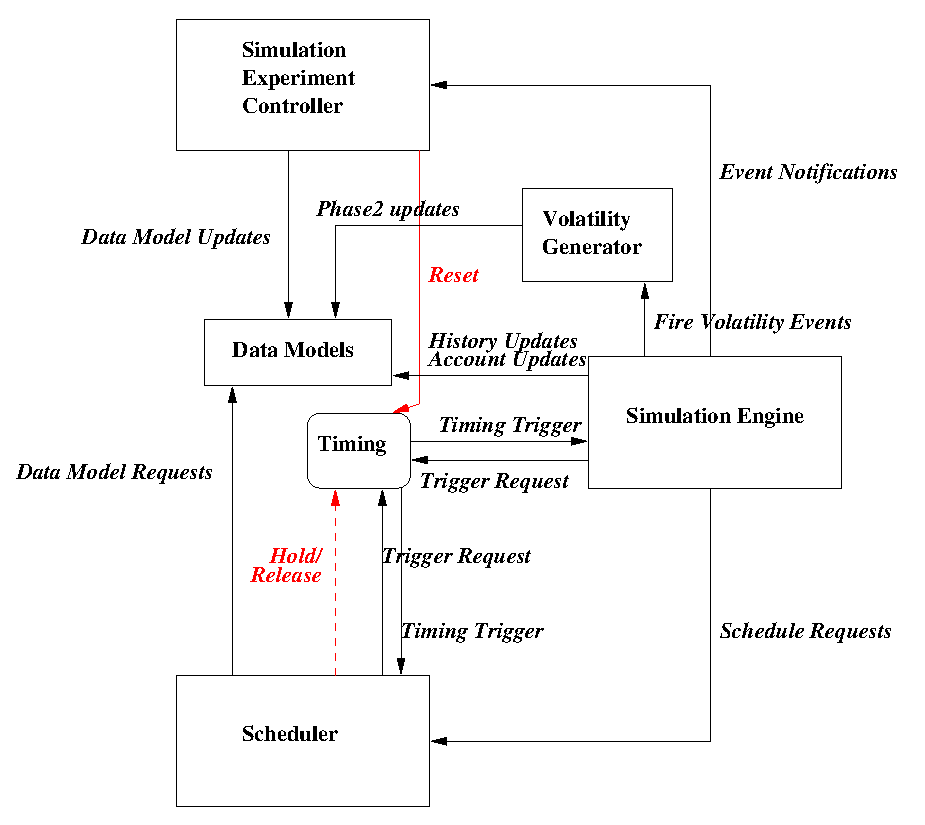
\includegraphics[scale=0.8, angle=0]{figures/sim_framework_arch.eps}
  \end{center}
  \caption[Architecture of the simulation framework.]
   {The simulation framework architecture. The Simulation Experiment Control application (SEC) is responsible for creating the various data models used by the scheduler. It invokes the simulator to run between specified times and receives feedback of significant scheduling events. The simulator makes scheduling requests of the scheduler and provides updates to the data models when the observations are deemed to have completed. Synchronization between components in speeded up simulation time is provided by the Time Signal Generator (TSG).}
  \label{fig:sim_frame_arch}
\end{figure}

The general format of a night's observing is in the form of a series of events. After each group has started executing there is generally nothing of significance capable of occuring from a scheduling point of view until the group completes or fails. To take advantage of this, the simulator is designed to operate by generation of discrete events. It had been anticipated that the time used in the model could simply be set to run at the maximum possible as permitted by the cycle of $schedule -> execute -> update$.

 However, because certain component operations within scheduler implementations might have to run as seperate threads (in the real world), there would have to be a form of time synchronization to allow these types of component to work correctly in the speeded up simulation environment. To illustrate by an example:

 A specific scheduler implementation might be required to run a sorting operation which takes perhaps 2 seconds of real time (a long time by simulation standards) every 5 minutes. Now 2 seconds of real time might actually correspond to several minutes or hours of simulation time, resulting in the sorting operation going \emph{out of phase} with the rest of the simulation. 

 This was solved by creating a Timing Signal Generator (TSG). This component permits several operations. In the main, an external client may request an asynchronous time-trigger at some future (simulation) time. The TSG keeps track of trigger requests and sends these signals out asynchronously to the requestors, in order, at the appropriate (simulation) times. Additionally, any client (thread) which requires to perform a \emph{significant} real-time operation may place a hold on the TSG to prevent any triggers being emitted. After completion of the real-time operation the client releases the hold and any queued triggers can be sent out. Ultimately, provided there are no extremely time-hungry real-time operations, the simulation clock advances significantly faster than real-time.

\subsection{Simulator Operation}
\label{ss:sim_ops}
The operation of the simulator cycle is described in Fig.~\ref{fig:ss_vgen_flowchart}. The simulator is controlled by an SEC and on initiation runs for a period specified by the SEC. With reference to the figure, a cycle of $schedule->execute->update$ is performed. Initially the simulation time $t$ is set to the start time specified by the SEC. A series of tests are then performed to determine \emph{what to do next} and \emph{how long} (denoted $\tau$) this operation will take in terms of simulation time. 

The first test determines if $t$ is during daytime. If so the simulation will skip forward to the calculated sunset time. If not, the second test determines if $t$ occurs during any scheduled \emph{disruptive} event (bad weather, mechanism failure, engineering time). If so the time will be advanced to the end of this disruption. If not, an observation group is requested from the schedule despatcher. If none are available, the simulation will skip forward by the length of a \emph{background observation} (effectively idle time). If a group is returned from the despatcher, the \emph{expected} execution time $\tau_{exec}$ is determined and a further test is performed to determine of any disruptive events are scheduled to start between $t$ and $t+\tau_{exec}$. If not, the simulation will be advanced to $t+\tau_{exec}$, otherwise to the start of the disruption $t+\tau_{sod}$. 

Once the advance ($\tau$) has been determined, but before the time is actually incremented, it is guaranteed that nothing can occur in this interval to affect the run of the simulation. At this point the Volatility Generator is called upon to effect any Phase 2 update events scheduled for the period $[t, t+\tau]$. The simulation time is then advanced by the relevant amount. If a group has been selected for execution it will have either succeeded or failed (it may have been aborted by a disruption event). The various models (history, accounting) are then updated and the SEC receives a notification from the simulator of group completion (or failure).


\begin{figure}[htbp]
\begin{center}
    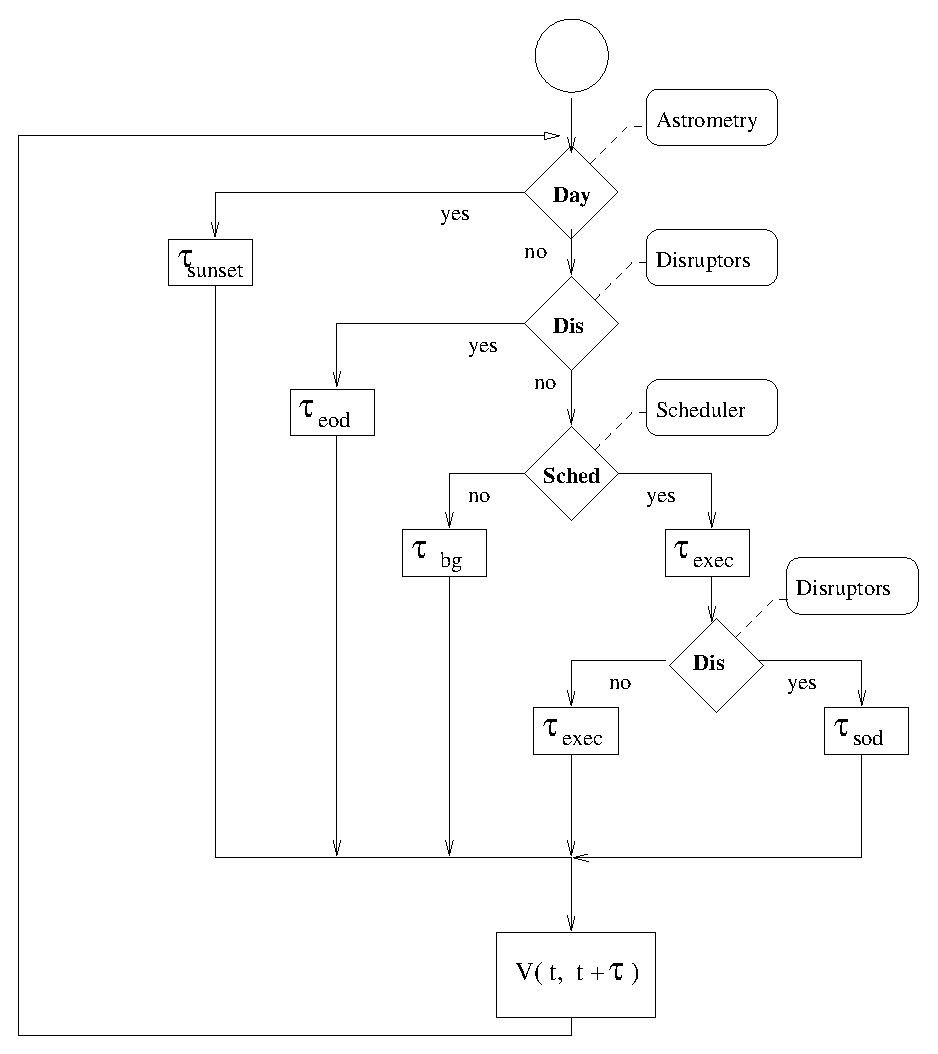
\includegraphics[scale=0.8, angle=0]{figures/ss_algorithm.eps}
\end{center}
\caption[Flowchart for simulation control algorithm.]
{Flowchart for simulation control algorithm. The time advance values in each cycle are: $\tau_{sunset}$ time remaining until sunset; $\tau_{eod}$ time until end of current disruption event; $\tau_{sod}$ time until start of next disruption event; $\tau_{bg}$ background observing time; $\tau_{exec}$ execution time of a group. The decision boxes represent the following tests:- \begin{inparaenum} [(\itshape i\upshape)] \item $Day(t)$ - is time $t$ daytime?, \item $Dis(t)$ - is time $t$ inside some disruption period ?, \item $Sched(t)$ - can the despatcher find anything to do at $t$?, \item $Dis(t, t+\tau)$ - are there any disruption events starting during the interval $(t, t+\tau)$. \end{inparaenum}. The volatility generator $V$ is invoked after each cycle to see if any volatile events should occur before the start of the next cycle.}
\label{fig:ss_vgen_flowchart}
\end{figure}


\subsection{Sources of uncertainty}
\label{sect:exp_uncertainty}
The real environment in which operational schedulers have to function provides many sources of uncertainty (Sect.~\ref{sect:env_components}). The simulation framework is intended to provide a controlled environment for the scheduler to run in but must provide a realistic degree of variation in these environmental variables. These sources of uncertainty affect both the complexity of the scheduling problem (in terms of complexity metrics) and the range of potential rewards possible (in terms of schedule quality metrics). The main stochastic inputs are:-

\begin{description}
\item [Stochastic execution model] The \emph{execution resource estimation model} (X) provides an estimate of the amount of time a group is expected to take. The various schedulers use this to decide when a group is likely to complete, however in reality a group might take more or less time due to various sources of uncertainty. The \emph{Stochastic execution model} allows the simulation framework to take these effects into account and introduces some variation in the simulated execution times of groups. This is generally implemented by using the prediction from X then adding some gaussian or white noise to simulate the effect of variable length telescope and instrument operations (Fig.~\ref{fig:simf_exec_timing_dist}).

\item [Environmental model] On an actual night the seeing and atmospheric extinction may vary over the full range and with a variety of timescales thus affecting the set of feasible groups available. This natural variation in the sky conditions are taken into account by the \emph{environmental model}.

\item [Phase 2 model] The distribution of the generator parameters used to create the Phase 2 information will affect the evolution of a schedule during the night since the Phase 2 model determines the range of groups available over time.

\item [Disruption model] Interruptions of varying sizes and lengths due to (unpredictable) events affect the degree of success of schedules, this aspect is simulated using a \emph{disruption model}.

\item [Volatility model] Evolution or volatility of the phase 2 database content is simulated using a \emph{volatility model} which allows new groups to be injected into the ODB at (controlled) random intervals thus affecting the contention and other parameters of the Phase 2 model.

\end{description}


\subsection{Scheduler implementations}
\label{ss:sched_impl}
Two different types of scheduler are used in the experiments. These take rather different views of the process.

\subsubsection{Despatch Scheduler}
\label{ss:sched_bds}
Despatch schedulers take a local view of optimization. At any point in time they will try to select the group $g$ which has the highest \emph{differential} score $f_g$ and which best matches current conditions. The algorithm is particularly straightforward:-

\begin{enumerate} 
\item The \emph{ExecutionFeasibilityModel} is used to generate a candidate list of groups which satisfy their timing constraints and all of their observing constraints under the current environmental conditions.

\item Using the \emph{ScoringModel}, various metrics and differential scores are calculated for each candidate group. 

\item The \emph{SelectionModel} is used to analyse the candidate metrics and choose one of these groups to execute.
\end{enumerate}

The baseline implementation used for simulations is called \emph{Basic Despatch Scheduler} (BDS\glossary{name={BDS},description={Basic despatch Scheduler - a simple scheduler}}). This implementation is typically configured to use different versions of \emph{SelectionModel} and \emph{ScoringModel}. For most cases the selection model $\xi_{BEST}$ is employed - this selects the highest scoring candidate group. Various biased selection models are tested in Sect.~\ref{sect:compsched}. The scoring model employed is a weighted sum of a number of standard metrics such that the differential score $f_g$ for a candidate group $g$ at time $t$ under environmental conditions $E$ is given by Eq.~(\ref{eq:weighted_score}):-

\begin{equation}
\label{eq:weighted_score}
f_g = \sum_{i} {w_i f_i(g,t,E)}
\end{equation}

The \emph{execution timing model} used by BDS has a configurable fixed duration estimate assigned to each type of observing sequence component (see Fig.~\ref{fig:group} in Sect.~\ref{sect:intro_background}) with the exception of exposures for which the duration is calculated using configurable, instrument-specific overheads. (See Table.~\ref{tab:exectime_factors} for more details.)


%  \breve{o} \vec{o}

\subsubsection{Look Ahead Scheduler}
\label{ss:sched_qlas}
%\newcommand{\echelon}{$\mathsf{\breve{e}chelon}$ }
%\newcommand{\echelons}{$\mathsf{\breve{e}chelons}$ }

%\newcommand{\echelon}{$\mathsf{sequence}$ }
%\newcommand{\echelons}{$\mathsf{sequences}$ }

\newcommand{\echelon}{sequence }
\newcommand{\echelons}{sequences }

The Look-Ahead Schedulers (LAS) try to increase the overall reward by optimizing over a period of time (global optimization). They have to make estimates of what is likely to happen in the future - both in terms of external conditions (stability, volatility, disruption) and the likely outcomes of their own actions (how likely are the selected groups to succeed, will they overrun). In the discussion to follow the term \echelon refers to the ordered sequence of groups to execute during a given horizon. A typical LAS implementation works as follows:-

\begin{enumerate}
\item The \emph{HorizonDeterminant}, using information about environmental stability, ODB volatility and disruption decides how long the \echelon horizon (H) should be. If the horizon is too short we risk losing potential reward. If H is too long, we risk breakages.

\item Using the \emph{SolutionGenerator}, a number of candidate \echelons are generated in which each group must satisfy the timing and observing constraints under the predicted conditions at its expected time of execution according to the \emph{ExecutionFeasibilityModel}.

\item The \emph{ScoringModel} and \emph{ExecutionTimingModel} are then used to calculate a potential reward ($F_S$) for each \echelon $S$. When we work out this score or reward, we are assume that conditions will not change during the duration of the sequence to de-enable any of the chosen groups, that the groups will not overrun and that the sequence will run to completion. This may not however turn out to be the case. 

In order to take into account such possibilities, one technique borrowed from AI is the concept of discounting, specifically the concept of Expected Future Reward (EFR)\glossary{name={EFR},description={Expected Future Reward - a method for discounting the value of potentially uncertain future rewards}}. In calculating potential reward, a discount rate ($\lambda$) is selected and applied to the scoring calculations to devalue contributions further into the future (later in the sequence). This derives from the notion that the value of a \emph{certain} reward right now outweighs the value of a potentially higher but uncertain reward at some time in the future. The further into the future and the more uncertain the potential reward, the less we value it. The choice of discounting rate is however the difficult part. 

If an EFR policy  is in force (Sect.~\ref{sect:architecture}) this would be used, perhaps in conjunction with environment and volatility prediction, to calculate the discount rate ($\lambda$). The discounted total reward $F_S$ for the \echelon is calculated using Eq.~(\ref{eq:discountreward}):-
\begin{equation}
\label{eq:discountreward}
F_S = \sum_{g \in S}{X_g f_g(t_g,e)e^{-\lambda (t_g-t_0)}}
\end{equation}
where $X_g$ is the expected execution duration of the group $g$, $f_g(t_g,e)$ is the differential score for $g$ at its expected time of execution $t_g$ under environmental conditions $e$ for a sequence starting at $t_0$. If EFR is not in use (as is the case for most of the experiments) then $\lambda \equiv 0$.

\item The \emph{SearchMechanism} examines the potential candidate \echelons to determine the one with the highest potential reward which is then selected for execution.

\item During execution, if conditions deteriorate, the \emph{BreakagePolicy} decides on the course of action to take. This might involve aborting the \echelon, swapping in some alternative groups or just carrying on.

\item If new or modified groups appear during execution, the \emph{SequestrationPolicy} determines whether these will be allowed to enter the \echelon. In a real-life scenario it might be that a very important and urgent group might be added at such a time. In particular if the horizon $H$ were very large (eg 4 hours) this new urgent group might well be missed

\item When a sequestration does takes place, the choice of which group(s) to replace is determined by a \emph{RetractionHeuristic}.

\end{enumerate}

Two implementations of LAS are employed in the simulation experiments.

\begin{itemize}
\item QLAS (Quantum Look Ahead Scheduler) \glossary{name={QLAS},description={Quantum Look-ahead Scheduler - a simple look-ahead scheduler using a random sequence generator}} uses a pre-assigned horizon length ($H$). Its solution generation proceeds by dividing the available horizon into discrete short time segments or \emph{quanta}, labelled $\tau_Q$). For each time quantum, a random selection is made from all those groups which are feasible at that time. For quanta in which no group is feasible an idle gap is left. Once the horizon is filled, the \echelon is scored and the highest scoring \echelon after a specified number ($N_S$) of runs is selected for execution. The operation of QLAS is such that during the execution of a schedule horizon any additional groups added cannot be considered until the horizon is completed - there is no \emph{SequestrationPolicy}. 

\item ELAS (Enhanced Look Ahead Scheduler) \glossary{name={ELAS},description={Enhanced Look-ahead Scheduler - a simple look-ahead scheduler based on QLAS but with a Sequestration Policy}} is a modified version of QLAS. The main enhancement is to allow new groups generated during execution to sequester time. The \emph{SequestrationPolicy} uses the mean differential score $\bar{q} = F_S/H$ of the groups included in the \echelon to calculate a threshold score value for the horizon. If a volatility event occurs during execution, the new group is checked to determine its feasibility window and differential quality metric $q_g$. These values along with the time remaining in the \echelon are compared to the pre-calculated threshold to decide if the group is allowed to be inserted into the \echelon by ejecting one or more previously included groups. The probability $P$ of inclusion of a group with score $q_g$ at time $t$ (measured from the start of the current \echelon of length H) and with feasibility window $W$ is given by Eq.~(\ref{eq:elas_sequester}).

\begin{equation}
\label{eq:elas_sequester}
  P = \left\{
    \begin{array}{l l}
     g(q_g,\bar{q},t,H) & \quad : q_g \geq \bar{q}\\
     0                  & \quad : q_g < \bar{q}\\
    \end{array} \right.
\end{equation}

where $g(q,\bar{q},t,H)$ is a rising function of $q_g-\bar{q}exp(-(1-W-(1+a)t)/H)$ with $g(0) = g_0$, $g(1) = 1$. The effect of this is to prevent groups of low score (relative to the mean score for the \echelon) from ejecting any sequenced groups early in the execution. As the execution procedes the threshold is eased so it becomes easier for a new group to jump in. Higher scoring groups are always more likely to be able to jump in than low scoring groups and ensures that groups which are capable of running in the next horizon are less likely to jump in than those which must run during just the current horizon. The swap or retraction rule is effected to allow one or more adjacent groups to be removed with just sufficient time to allow the new group to run but with as little lost time as possible and with the minimum loss of reward as follows:-

%\renewcommand{\labelitemii}{$\triangleright$}

\begin{itemize}  
  \item Determine if any single groups of duration $X_1 >= X_g$ exist. 
  \item If so, record the one for which ($X_1/X_g-1)X_1f_1$ is smallest.
  \item Determine if any adjacent pairs of group exist such that $X_1+X_2 >= X_g$.
  \item If so, record the pair for which $((X_1+X_2)/X_g-1)(X_1f_1+X_2f_2$) is smallest.
  \item Continue to triples and quadruplets etc of groups, recording the lowest scaled reward in each category.
  \item Finally, select the single, pair or higher grouping with the lowest loss of total reward.
\end{itemize}

\end{itemize}

\subsection{Notes on notation used in results}

In the following chapters results of simulations are displayed mainly in the form of graphs showing differences in various quality metrics achieved by different schedulers or scheduler variants against some independant variable.

A particular form of graph frequently used is the \emph{candlestick} or \emph{box and whisker} plot. A typical example is shown in Fig.~\ref{fig:bdsqel}. In these plots the box area is centred vertically on the average result for the dependant variable for the given independent variable. The upper and lower limits of the box represent the average value $\pm $ one standard deviation of the simulation results. The extension bars above and below the box represent the individual extreme values of the dependant variable found during the simulations.

The statistics derived from the graphed results are found in Appendix~\ref{sect:app_stats}. The majority of the derived tables show the value of the difference in a quality metric between one or more comparison schedulers against the results for some baseline scheduler at a variety of selected values of the independant variable used. These \emph{x} values are typically chosen to display a particular feature of the results, e.g. where a  plot suddenly rises from a steady low value followed by a typical data point in the risen region of the graph.

 The main statistical values shown in the tables are the values of\notation{name={$\Delta_{90}(C,B)$},description={Fractional improvement in quality of $C$ over $B$},sort={D}} $\Delta_{90}(C,B)$. This represents the improvement in quality ($Q$) for the comparison model ($C$) relative to the baseline model ($B$). It is in fact the ratio of the mean difference between the chosen quality metric $Q_C$ of the comparison and of the baseline $Q_B$ relative to the baseline measurement. The second figure in each table cell, in parenthesis, is the range of this variable in which 90\% of results are expected to lie. e.g. $\Delta_{90}(C,B) = 25 (\pm 5)$ indicates that 90\% of the results for $(Q_C-Q_B)/Q_B$ lie between 20\% and 30\% or that $C$ is between 20\% and 30\% better than $B$.


% EX MAM
\section{Man against machine}
\label{sect:mam_study}
\subsection{Introduction}Selecting appropriate groups to perform is a complex task. There are many trade-offs to be made between the various competing preferences and constraints. When the schedule is heavily loaded, i.e. there are potentially more observations to perform than could be accomodated even under ideal conditions, the job of the scheduler becomes both simpler and more difficult. It is relatively \emph{easy} to find a solution which satisfies the constraints, however finding an optimal solution is rendered more \emph{difficult} due to the number of potential solutions to compare. 

A major problem is to determine just what those trade-offs are. We would like to be able to answer questions like:- \emph{how much more important is a high priority, non-urgent group relative to a medium priority, urgent group?} It is because it is difficult to quantify these relative weights that we turn to the human scheduler. Humans are capable of processing this type of complex, interlinked information and making these sort of trade-offs on a daily basis - often with little knowledge they are doing it. If we set up a human to perform the task we might be able to deduce from what they have done and the choices they have made some of the rules they are using (often without realizing) and the relative weightings they employ. 

Two sets of trials are performed. Firstly the human scheduler (referred to as HS) is presented with a snapshot of the ODB content for the trial night in a tabular format from which to generate a schedule. Secondly a set of simulations are run in which the relative scoring weights are changed to try and reproduce the results of HS and, \emph{if possible}, to beat them.

\subsection{Characterization of problem}
On the night of the test (13-14 November 2007) there are some 13.33 hours of night (including twilight time) with additonal details in Table.~\ref{tab:mam_nights}.
The supplied ODB snapshot consists of 131 groups and a total of 2880.32 minutes (48 hours) of available observing time in the night, an oversubscription factor of 3.6

\begin{table}[htbp]
\begin{center}
\begin{tabular}{lll}
\toprule
\multicolumn{3}{c}{Case study night characteristics} \\
\midrule
Item       &  Time               & Lunar elevation \\
\midrule
Sunset     & 2007-11-13 18:15 UT & 23.4$^{\circ}$\\
StartNight & 2007-11-13 19:40 UT & 11.2$^{\circ}$\\
Moonset    & 2007-11-13 20:50 UT & 0.0$^{\circ}$\\
EndNight   & 2007-11-14 06:05 UT & -66.0$^{\circ}$\\
Sunrise    & 2007-11-14 07:35 UT & -47.3$^{\circ}$\\
\midrule
Item                         & Duration (hours) \\
\midrule
Length of dark night         & 10.42\\
Length of night inc twilight & 13.33\\
\bottomrule
\end{tabular}
\caption[Characteristics of test night for HS1 experiment]{Characteristics of the test night for HS1 experiment.}
\label{tab:mam_nights}
\end{center}
\end{table}


The groups within the snapshot are distributed throughout the range of priority as shown in Table~\ref{tab:priority_distrib}. Excluding the background groups, which should only run as a last resort and do not contribute to the science program, there are a total of 34.8 hours giving a more realistic oversubscription factor of 2.6.

% GROUP PRIORITY DISTRIBUTION
\begin{table}
\begin{center}
\begin{tabular}{llp{6cm}}
\toprule
\multicolumn{3}{c}{ODB snapshot characteristics} \\
\midrule
Priority & $N_G$ & $\sum{X_g}$ (hours)\\
\midrule
0 & 1 & 2.8\\
1 & 55 & 1190.1\\
2 & 26 & 462.3\\
3 & 12 & 169.5\\
5 & 2  & 39.4\\
BG & 23 & 790.3\\
STD & 12 & 226.8\\
\midrule
Total & 131 & 2880.3\\
\bottomrule
\end{tabular}
\caption[Distribution of number of groups between priority levels for HS1 experiment]{Distribution of number of groups $N_G$ and total executable time $\sum{X_g}$ among the available priority levels. Low priority (1 and 2) make up the bulk of the science groups with relatively few high priority (5) groups. Background (BG) groups which only execute if no others are available and calibration standard (STD) groups are not part of the science program.}
\label{tab:priority_distrib}
\end{center}
\end{table}

Figures~\ref{fig:mam_h1_contention} and \ref{fig:mam_h1_dmd} show respectively the contention and demand plots for the night. The predicted contention $C_c$ is very high at around 90 for much of the night. A simulation run with a \emph{typical} scheduler, shown on the same plot shows the actual contention dropping from around 80 to 40 over the course of the night. The total demand $C_d$ remains fairly constant at a level of around 4 to 5 for the night while the urgency-weighted demand $C_{ud}$ rises from 1 to nearly 2 over the course of the night. This latter indicates that selection of just the urgent groups would likely fill most of the available observing time.

\begin{figure}[htbp]
\begin{center}
    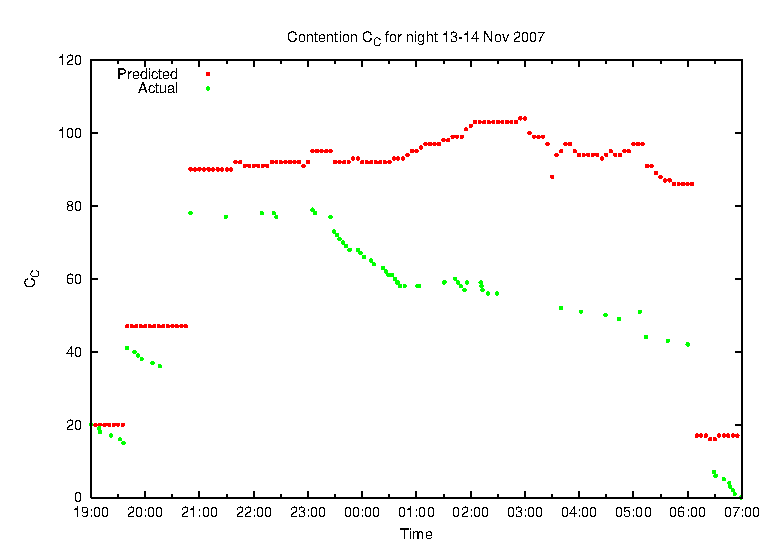
\includegraphics[scale=1.0, angle=0]{figures/mam/cont.eps}
\end{center}
\caption[Contention for night 13-14 November 2007.]
{Contention for night 13-14 November 2007 for HS1 test. The two plots show the expected contention ($C_C$) based on ODB content calculated in advance and the actual contention ($C_A$) derived during a typical scheduling run on the night. $C_A$ displays the typical staircase behaviour as the pool of observations is depleted during the night.}
\label{fig:mam_h1_contention}
\end{figure}

\begin{figure}[htbp]
\begin{center}
    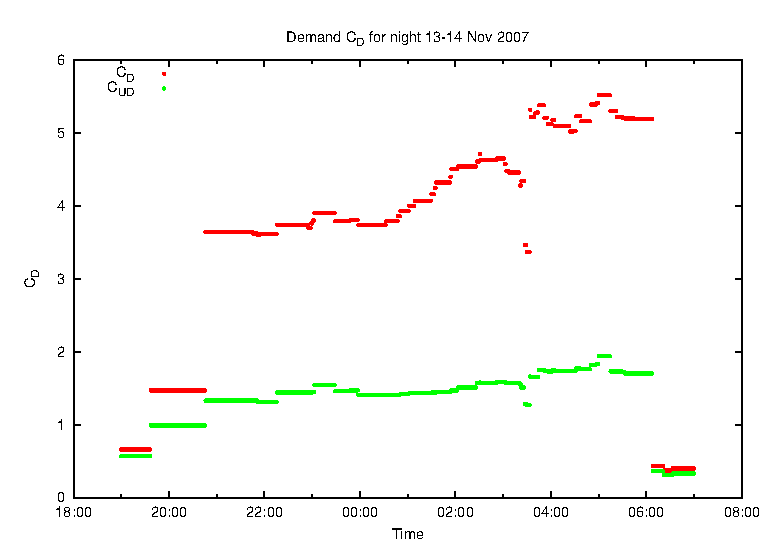
\includegraphics[scale=1.0, angle=0]{figures/mam/dmd.eps}
\end{center}
\caption[Demand for night 13-14 November 2007.]
{Demand for night 13-14 November 2007 for HS1 test. The two plots show the overall demand ($C_D$)and urgency-weighted demand ($C_{UD}$). As can be seen there are enough urgent observations to fill the night.}
\label{fig:mam_h1_dmd}
\end{figure}


\subsection{Human scheduling trial (HS1)}
A human subject (expert scheduler) is provided with information concerning which groups are potentially feasible on the test night. An example section of the data provided is shown in Table.~\ref{tab:example_gen}. The information, described in Table.~\ref{tab:hsgexample} contains details of the target, timing and observing constraints along with a simple pre-calculated feasibility plot for the night for each group. Some metrics are also available. The urgency metric indicates on how many remaining nights the group might be observed. The execution-time metric indicates the expected execution time of the group. 

In light of the difficulty for a human to generate the schedule by collating the considerable amount of information available a number of the normal constraints were relaxed. e.g. it is not easy for a human to keep precise track of the accumulating time to the second so execution times are given to the nearest minute. The accuracy of the availability plot is also shown only to around 5-10 minutes so when testing the feasibility (in terms of target elevation) a few degrees of leeway are given. In order to uncomplicate the scenario the assumption is also made that seeing is good for the whole night. 

The HS uses the information to devise a schedule for the night by recording the start time and ID of each group to execute in order. Due to the time taken to perform one of these HS trials - several hours, only a single trial (HS1) was performed.


\begin{table}
\begin{center}
\begin{tabular}{lllp{6cm}}
\toprule
\multicolumn{4}{c}{Description of the columns in the table provided to the human scheduler} \\
\midrule
{\bf Column} & {\bf Title}  & {\bf Example} & {\bf Description}\\
\midrule
1  & Numeric ID     & G\_476          & Used by HS to mark up the schedule.\\
2  & Target RA      & 0:42:49.64      & RA (hh:mm:ss) format.\\
3  & Target Dec     & 41:15:26.50     & Declination (dd:mm:ss) format.\\
4  & Group Name     & ANGM31          & Name of the group.\\
5  & Timing         & MONITR 2.5H [2] & Timing constraint class.\\
6  & Moon OC        &                 & Observability with moon risen.\\
7  & Seeing OC      & POOR            & Minimum seeing category.\\
8  & Solar Elev OC  &                 & Observability in twilight.\\
9  & Priority       & 2               & TAG assigned priority.\\
10 & Execution Time & 33.4M           & Expected time to run.\\
11 & Urgency        & CRIT              & Remaining observable nights.\\
12 & Availability   & \_\_9**********\_ & Display of observability. \\
\bottomrule
\end{tabular}
\caption[Description of the columns in the table provided to the human scheduler]
{Description of the columns in the table provided to the human scheduler. In the observing constraint (OC) columns, the absence of a label means \emph{no constraint}. The timing constraints include FLEX (flexible - one off), MONITOR (monitor with period and window size (hrs)), INTVL (minimum-interval with interval size(hrs)). If the group \emph{must} be observed tonight (urgency = 1 night) this is shown as either CRIT or ICRIT (minimum-interval groups are never \emph{entirely} critical as they do not also specify a maximum interval). The availability column shows when a group is feasible through the night. Each symbol represents 1/14th part of the night and indicates depending on the symbol what fraction of that period the group can be observed. - (none of period), 9 ($<90$\% of period), * ($<100$\%) }.
\label{tab:hsgexample}
\end{center}
\end{table}


\subsection{Results of HS1 trial}
The analysis proceeds as follows:- For each scheduled (group ID, start-time) pair, the feasibility is worked out for that time. This consists of testing the target elevation against dome limit (20 degs) and the group constraints on moon and sun elevation against actual elevations. If the schedule is feasible, the various quality metrics are then computed.

The HS1 experiment yielded a run of 147 group executions. There were a total of 9 overruns of respectively (1,1,1,1,3,4,5,10,10) minutes, these were considered sufficiently minor to be ignored. A preliminary look at the scoring profile shows the value of $elevation/transit\_height$ to be generally high - suggesting the human scheduler has tried to observe targets as they cross the zenith. There are 2 instances of targets observed below the horizon - one of these at -60 degrees elevation ! - possibly a misreading of a declination? This value was removed from the final results to avoid skewing.

\clearpage

\begin{landscape}

\begin{table}[h!]
  \begin{center}
  \end{center}
  \caption{Sample section of table available to HS. Description of these columns are found in Table.~\ref{tab:hsgexample}}
  \label{tab:example_gen}
\end{table}

\scriptsize
\begin{verbatim}

G_276     3:24:44.055  50:11:21.63  com17Pmon-071030    MONITR 48H [36]                     POOR ASTR  P= 1   XT= 2.25M    RN= CRIT 3***********9_
G_355     3:13:24.16   18:49:38.40  FS109               MONITR 3H [1]                       POOR ASTR  P= STD XT= 4.6M     RN= CRIT _5*********7__
G_369     3:24:7.995   50:9:33.39   17P-mosaic          FLEXBL                              AVER ASTR  P= 3   XT= 13.73M   RN= 21   3***********9_
G_370     3:24:7.995   50:9:33.39   17P-monitor         MONITR 3H [2]                       AVER NAUT  P= 2   XT= 3.63M    RN= CRIT 3***********9_
G_025     4:9:17.00    30:46:33.00  932a000t000         FLEXBL                         DARK POOR       P= 1   XT= 3.27M    RN= 17   __9**********_
G_028     4:30:14.00   35:16:10.00  927e000t000         FLEXBL                         DARK POOR       P= 1   XT= 3.27M    RN= 17   __7**********5
G_093     5:34:32.00   22:0:52.00   927h000t000         FLEXBL                         DARK POOR       P= 1   XT= 3.27M    RN= 16   ___2**********
G_382     5:5:30.60    52:49:54.00  zero_G191B2         MONITR 5H [3]                       POOR       P= STD XT= 3.53M    RN= CRIT __7***********
G_048     6:54:18.125  24:40:7.32   725d000t000         FLEXBL                              POOR ASTR  P= 1   XT= 1.27M    RN= 19   _____*********
G_408     6:54:18.12   24:40:7.38   927c000t000         FLEXBL                              POOR ASTR  P= 2   XT= 1.27M    RN= 19   _____*********
G_002     7:24:18.00  -0:32:17.00   Photom_G1_RU149     INTVAL 3H                           POOR ASTR  P= STD XT= 9.87M    RN= ICRT ______6*******
G_126     7:8:0.77     22:31:14.50  FocusShort_07       MONITR 168H [167]                   POOR ASTR  P= BGR XT= 7M       RN= 7    _____7********
G_284     7:23:44.00   20:25:6.00   mho_monitor         INTVAL 22.5H                        POOR       P= 1   XT= 71.1M    RN= ICRT _____4********
G_352     7:24:14.40  -0:33:4.10    FS14                MONITR 3H [1]                       POOR ASTR  P= STD XT= 5.43M    RN= CRIT ______6*******
G_371     7:36:51.00   65:36:7.00   lens_2403           MONITR 48H [36]                     POOR       P= 2   XT= 15.07M   RN= CRIT ____9*********
G_259     8:6:11.10   -27:31:42.00  ESO494-G26          FLEXBL                         DARK POOR       P= 1   XT= 22.17M   RN= 11   ________4*****
G_358     8:6:23.70    20:6:31.90   J0806               INTVAL 96H                          POOR       P= 3   XT= 27.33M   RN= 17   ______6*******
G_472     8:54:48.90   20:6:30.64   0851                MONITR 168H [167]              DARK AVER       P= 1   XT= 7.8M     RN= 3    _______8******
G_237     9:17:21.90   41:54:38.00  UGC4904             FLEXBL                         DARK POOR       P= 1   XT= 22.17M   RN= 13   ______1*******
G_260     9:32:6.20    8:26:31.00   NGC 2906            FLEXBL                         DARK POOR       P= 1   XT= 23.83M   RN= 12   ________8*****
G_263     9:45:48.30  -14:22:6.00   NGC2993             FLEXBL                         DARK POOR       P= 1   XT= 22.17M   RN= 10   _________7****
G_266     9:54:28.60  -25:42:12.00  NGC3054             FLEXBL                         DARK POOR       P= 1   XT= 23.83M   RN= 9    __________8***
G_280     9:50:31.97  -2:49:47.20   group07b01c         FLEXBL                         DARK AVER       P= 1   XT= 28.8M    RN= 11   ________1*****
G_281     9:47:51.21  -2:24:18.80   group07b01b         FLEXBL                         DARK AVER       P= 1   XT= 28.8M    RN= 11   ________2*****
G_373     9:55:33.20   69:3:55.00   lens_M81            MONITR 48H [36]                     POOR       P= 2   XT= 15.07M   RN= CRIT ______8*******
G_004     10:50:5.70  -0:1:12.00    Photom_G1_1047+003  INTVAL 3H                           POOR ASTR  P= STD XT= 9.63M    RN= ICRT _________2****
G_265     10:52:11.40  32:57:2.00   NGC 3430            FLEXBL                         DARK POOR       P= 1   XT= 23.83M   RN= 11   ________3*****
G_282     10:11:42.74 -2:58:16.90   group07b01d         FLEXBL                         DARK AVER       P= 1   XT= 28.8M    RN= 10   _________8****
G_407     10:39:57.45  10:4:0.47    926j000t000         FLEXBL                              POOR ASTR  P= 2   XT= 1.31M    RN= 19   _________8****

                  Small sample of the table available to human scheduler. The full table has 137 rows. Rows are ordered by the RA
                  of the group's target as can be seen in the final (observability) column. 
\end{verbatim}
\end{landscape}
\normalsize

%G_213     11:32:2.40   36:41:53.00  UGC6517             FLEXBL                         DARK POOR       P= 1   XT= 22.17M   RN= 10   _________7****
%G_244     11:25:2.50  -9:47:43.00   NGC3672             FLEXBL                         DARK POOR       P= 1   XT= 22.17M   RN= 9    __________2***
%G_353     11:37:5.15   29:47:58.40  FS21                MONITR 3H [1]                       POOR ASTR  P= STD XT= 5.43M    RN= CRIT _________4****
%G_204     12:52:34.70 -9:46:36.00   MCG-01-33-34        FLEXBL                         DARK POOR       P= 3   XT= 23.83M   RN= 4    ____________8*
%G_210     12:5:34.20   50:32:21.00  NGC4088             FLEXBL                         DARK POOR       P= 1   XT= 22.17M   RN= 10   _________6****
%G_218     12:2:12.20   62:8:14.00   NGC4041             FLEXBL                         DARK POOR       P= 1   XT= 22.17M   RN= 11   ________2*****
%G_245     12:48:13.60 -3:19:58.00   NGC4691             FLEXBL                         DARK POOR       P= 1   XT= 23.83M   RN= 9    ___________1**
%G_439     13:6:56.00   29:34:48.00  z2_1_H13            MONITR 672H [599.98]           DARK POOR       P= BGR XT= 49.73M   RN= 5    ___________9**
%G_440     13:6:56.00   29:34:48.00  z1_1_H13            MONITR 672H [599.98]           DARK POOR       P= BGR XT= 49.73M   RN= 5    ___________9**
%G_360     14:6:24.82   61:26:40.90  J1406               INTVAL 72H                          POOR       P= 3   XT= 27.33M   RN= 21   2_________1***
%G_481     14:17:59.60  25:6:53.00   5548_opt            MONITR 168H [120]                   POOR ASTR  P= 2   XT= 3.13M    RN= 3    ____________6*
%G_427     16:35:15.49  38:8:4.50    darkbias_16h        MONITR 24H [22.97]                  POOR ASTR  P= 2   XT= 4.34M    RN= CRIT *7____________
%G_275     17:57:48.00  4:42:48.50   TST-BarnStar-071105 FLEXBL                              POOR       P= 0   XT= 2.8M     RN= 10   **____________
%G_365     19:0:34.78   22:34:54.10  Focus19_zr          INTVAL 12H                          AVER CIVT  P= BGR XT= 9.9M     RN= ICRT ***7__________
%G_366     19:0:34.78   22:34:54.10  Focus19_rr          INTVAL 168H                         AVER CIVT  P= BGR XT= 9.8M     RN= 21   ***7__________
%G_367     19:0:34.78   22:34:54.10  Focus19_Br          INTVAL 12H                          AVER CIVT  P= BGR XT= 11.18M   RN= ICRT ***7__________


\subsection{Simulation trials}
Several simulation trials were performed using a basic despatch scheduler (BDS) and several configurations of a look-ahead scheduler (QLAS). The BDS simulations were performed using different weighted scoring functions. The QLAS simulations were performed using horizons of 1, 2, 4 and 8 hours and using search parameters of 100, 250 and 2500 trials. Each simulation was run 100 times to obtain statistical values for the various Q metrics.

A first set of trials were run using the scoring function $w_{el}f_{el}+(1-w_{el})f_{pr}$ with $w_{el}$ ranging from 0.0 to 1.0. With $w_{el}=0$ the scoring is purely based on priority. At the other extreme ($w_{el}=1$) the scoring is purely based on target elevation. Plots of the quality metrics $Q_{el}$ and $Q_{pr}$ against $w_{el}$ are shown in Figures.~\ref{fig:bdsqel} and \ref{fig:bdsqpr} with accompanying statistics in Tables~\ref{b:f73a} and \ref{b:f73b}. 

The results of HS1 and BDS simulations with a random selection model are plotted for comparison. From Fig.~\ref{fig:bdsqel} it is clear that random selection is always a poorer option. The HS wins over BDS (29.4\% $\pm 4$\%) when $w_{el}$ is small (priority-dominated selection) and only after $w_{el}>0.9$ is BDS better (17.5\% $\pm 3$\%) - this suggests that the HS is quite elevation-dominated. Inspection of Fig.~\ref{fig:bdsqpr} shows again that random selection is a poor choice. However we also see that HS beats BDS only when $w_{el}$ exceeds 0.7, suggesting that HS has a lower degree of priority bias. From this we may conclude that HS is using a scoring criterion with a large value of $w_{el}$ and a somewhat lower value of $w_{pr}$ though it is not feasible to determine exactly what these are.

A further series of simulations were performed using BDS with fixed values of $w_{el}$ and $w_{pr}$ to gauge the variation in results. The results for these are shown in Table.~\ref{tab:hsbdscomp}. The column labelled {\bf h1} represents HS1. The various columns labelled $\mathbf{B_a}$ represent the use of BDS with scoring based solely on metric $f_a$. The columns $\mathbf{B_{x,y}}$ represent BDS scored using a combination of $f_{pr}$ and $f_{el}$ in the proportion $(xf_{el}+yf_{pr})/10$. 

The scheduler $B_{el}$ achieves the best results for $Q_{el}$ as might be expected. Interestingly it performs slightly less well than HS on $Q_{rn}$ and $Q_{td}$, and indeed HS performs better on this metric than any BDS implementations including $B_{rn}$. This suggests there may be an element of \emph{urgency-weighting} in HS. $B_{pr}$ performs best on $Q_{pr}$, however, surprisingly slightly less well than HS overall on this metric. HS holds its own against all the BDS implementations on the other quality metrics with the exception of $Q_{td}$ where $B_{td}$ performs twice as well as anything else. 

\begin{figure}[htbp]
  \begin{center}
    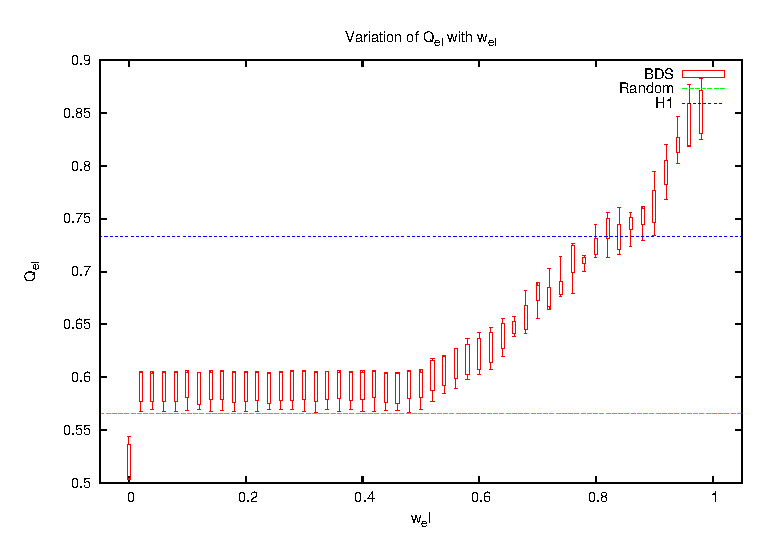
\includegraphics[scale=1.0, angle=0]{figures/cmp_el.eps}
  \end{center}
  \caption[Variation of $Q_{el}$ with $w_{el}$ for BDS simulations.]
  {Variation of $Q_{el}$ with $w_{el}$ for BDS simulations with scoring funtion $w_{el}f_{el}+(1-w_{el})f_{pr}$. Plots labelled \emph{H1} and \emph{Random} represent the results for HS1 and for BDS with a random selection model.}
  \label{fig:bdsqel}
\end{figure}
  
\begin{figure}[htbp]
  \begin{center}
    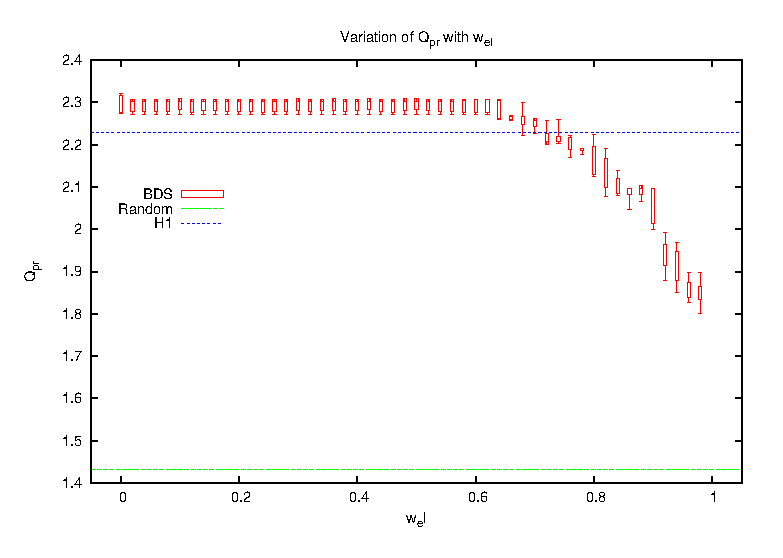
\includegraphics[scale=1.0, angle=0]{figures/cmp_pr.eps}
  \end{center}
  \caption[Variation of $Q_{pr}$ with $w_{el}$ for BDS simulations.]
  {Variation of $Q_{pr}$ with $w_{el}$ for BDS simulations with scoring funtion $w_{el}f_{el}+(1-w_{el})f_{pr}$. Plots labelled \emph{H1} and \emph{Random} represent the results for HS1 and for BDS with a random selection model.}
  \label{fig:bdsqpr}
\end{figure}
 
\begin{table}[p]

  \subtable [Results of BDS simulations and Human scheduler] {
    \label{tab:hsbdscomp}
    \begin{tabular}{|l|rrrrrrrrr|}
     \hline
     {\bf metric} & {\bf $h_1$} & {\bf $B_{el}$} &  {\bf $B_{pr}$} & {\bf $B_{rn}$} & {\bf $B_{td}$} & {\bf $B_{2,8}$} & {\bf $B_{5,5}$} & {\bf $B_{8,2}$} & {\bf $B_{rnd}$}\\
     \hline
     {\bf $Q_{el}$} & 0.77 & 0.88 & 0.52 & 0.36 & 0.4  & 0.59 & 0.58 & 0.72 & 0.56 \\
     {\bf $Q_{pr}$} & 2.34 & 1.87 & 2.29 & 1.73 & 1.54 & 2.3  & 2.3  & 2.16 & 1.43 \\
     {\bf $Q_{sm}$} & 0.28 & 0.3  & 0.26 & 0.28 & 0.32 & 0.25 & 0.25 & 0.25 & 0.33 \\
     {\bf $Q_{lm}$} & 0.71 & 0.8  & 0.68 & 0.82 & 0.92 & 0.64 & 0.63 & 0.7  & 0.86 \\
     {\bf $Q_{rn}$} & 0.67 & 0.48 & 0.4  & 0.58 & 0.4  & 0.47 & 0.47 & 0.45 & 0.35 \\
     {\bf $Q_{td}$} & 0.07 & 0.06 & 0.05 & 0.1  & 0.12 & 0.06 & 0.06 & 0.05 & 0.08 \\
     {\bf $Q_{xt}$} & 0.99 & 0.99 & 0.96 & 0.99 & 1.0  & 0.96 & 0.97 & 0.96 & 1.0  \\
     \hline
   \end{tabular}
  }

%\subsection{LAS simulation results}
%extra features - bg selection thresh - other wise stay idle, overun thresh frac of group in horizon

  \subtable [Results of LAS simulations and Human scheduler (n=100)] {
    \label{tab:lascomp1}
    \begin{tabular}{|l|r|rrrr|}
      \hline
     {\bf metric} & {\bf $h_1$} & {\bf 1} & {\bf 2} &  {\bf 4} & {\bf 8} \\
     {\bf $Q_{el}$} & 0.77 & 0.574 &0.569 &0.579 &0.571\\
     {\bf $Q_{pr}$} & 2.34 & 1.848 &1.801 &1.811 &1.812\\
     {\bf $Q_{sm}$} & 0.71 & 0.815 &0.820 &0.847 &0.839\\
     {\bf $Q_{lm}$} & 0.28 & 0.317 &0.321 &0.325 &0.327\\
     {\bf $Q_{rn}$} & 0.67 & 0.362 &0.344 &0.347 &0.358\\
     {\bf $Q_{xt}$} & 0.99 & 1.000 &0.998 &1.012 &1.007\\
     \hline
    \end{tabular}
  }

  \subtable [Results of LAS simulations and Human scheduler (n=500)] {
    \label{tab:lascomp2}
    \begin{tabular}{|l|r|rrrr|}
      \hline
      {\bf metric} & {\bf $h_1$} & {\bf 1} & {\bf 2} &  {\bf 4} & {\bf 8} \\
      {\bf $Q_{el}$} &  0.77 & 0.569 &0.576 &0.584 &0.584\\
      {\bf $Q_{pr}$} & 2.34  &1.863 &1.818 &1.790 &1.807\\
      {\bf $Q_{sm}$} &  0.71 &0.816 &0.831 &0.838 &0.843\\
      {\bf $Q_{lm}$} & 0.28  &0.311 &0.326 &0.329 &0.330\\
      {\bf $Q_{rn}$} & 0.67  & 0.345 &0.357 &0.356 &0.344\\
      {\bf $Q_{xt}$} & 0.99  &0.994 &1.010 &1.016 &1.011\\
      \hline
    \end{tabular}
  }

  \subtable [Results of LAS simulations and Human scheduler (n=2500)] {
    \label{tab:lascomp3}
    \begin{tabular}{|l|r|rrrr|}
      \hline
      {\bf metric} & {\bf $h_1$} & {\bf 1} & {\bf 2} &  {\bf 4} & {\bf 8} \\
      {\bf $Q_{el}$} &  0.77 & 0.573 &0.577 & 0.58 & 0.582\\
      {\bf $Q_{pr}$} & 2.34  &1.855 &1.826 & -&-\\
      {\bf $Q_{sm}$} &  0.71 &0.837 &0.838 & -&-\\
      {\bf $Q_{lm}$} & 0.28  &0.324 &0.327 & -&-\\
      {\bf $Q_{rn}$} & 0.67  &0.340 &0.342 & -&-\\
      {\bf $Q_{xt}$} & 0.99  &1.013 &1.011 & -&-\\
      \hline
    \end{tabular}
  }
\end{table}

\subsection{Summary and conclusions}
It has been shown that a human scheduler using rules which may not be known to the scheduler himself is capable of generating effective, high-quality schedules as measured by various Q metrics. In some cases the human scheduler was able to outperform an automated (BDS) scheduler on certain metrics. Inspection of the table columns shows the scheduler $B_{8,2}$ comes fairly close to matching the HS column suggesting the relative weightings used are given approximately by $0.8 f_{el} + 0.2 f_{pr}+ \epsilon f_{rn}$ where $\epsilon$ is very small ($\ll 0.1$).

% EX SCORING
\section{Investigation of effects of varying scoring weights}
\label{sect:exp_scoring}
\subsection{Introduction}

This investigation involves running a series of one-night simulations under different environmental assumptions to see the effect of varying the relative values of the scoring heuristic weights. The rational behind this investigation is to provide some initial insight into the usefulness of the various \emph{Schedule Quality Metrics} (SQM) and to provide a shakedown test of the simulation framework on real data. By selecting 2 seperate but similar nights (in terms of loading) it should be possible to get a preliminary idea on the range of likely values and variation of these metrics.


\subsection{Method}
Two nights were considered and are detailed in Table.~\ref{tab:scoring_nights}. On night \emph{$^\#$1} (27th-28th September 2007), the moon rises early and is up for the full night. There are  12 hours of night of which 9.5 hours are astronomically dark. Night \emph{$^\#$2} (3th-4th November 2007) has 5.5 hours of lunar dark time at the start of the night during the 13.0 hour night of which 10.2 hours are astronomically dark.

 A series of simulations were run for fixed environmental scenarios $E_{FX}$ (fixed, excellent seeing) and $E_{FP}$ (fixed, poor seeing) on each of the two nights. The scoring model was chosen to be:-

\begin{equation}
\label{eq:two_score}
  f_g = w_{trans} f_{trans}(g,t,E) + w_{px} f_{px}(g,t,E)
\end{equation}

The weights of the \emph{transit elevation} function $w_{trans}$ and the \emph{execution priority} function $w_{px}$ were varied for each set of 1000 simulations such that $w_{trans} + w_{px} = 1$. These two functions were chosen as they are generally (operationally) the highest weighted functions and because $f_{px}$ does not vary in time whereas $f_{trans}$ does vary with time for a given group. No other functions were incorporated into the scoring calculation in order to avoid any unnecessary noise.

The SQMs used to evaluate the quality of the resulting schedules are $Q_{OA}$ - the optimal airmass metric, $Q_{PX}$ - the execution priority metric, $Q_{RN}$ - urgency metric, $Q_{TD}$ - demand metric, $Q_{PX \cdot OA}$ - priority weighted optimal airmass and $Q_{XT}$ the total execution time as a fraction of available night. 

In addition, for each set of simulation parameters an additional set of simulations were performed using a random selection from the available feasible groups.

\begin{table}[htbp]
\begin{center}

\begin{tabular}{lll}
\toprule
\multicolumn{2}{c}{Case study night characteristics} \\
\midrule
Item & Night 1 & Night 2 \\
\midrule
Date                & 27-28 Sep 2007 & 3-4 Nov 2007\\
Sunset              & 18:59 UT         & 18:22 UT\\
Sunrise             & 06:59 UT         & 07:21 UT\\
Start Astro night   & 20:17 UT         & 19:42 UT\\
End Astro night     & 05:41 UT         & 06:01 UT\\
Moonset             & 08:43 UT          & 14:55 UT\\
Moonrise            & 19:23 UT          & 01:37 UT\\
\midrule
Length of night(hh:mm)        & 12:02   & 12:59\\
Length astro night(hh:mm)     & 9:24    & 10:19\\
Length astro moon dark(hh:mm) & 0:0     & 5:56\\
Lunar dark fraction & 0.0\%   & 58.8\%\\
\bottomrule
\end{tabular}
\caption[Case study night characteristics for scoring experiments]
{Case study night characteristics for scoring experiments.}
\label{tab:scoring_nights}
\end{center}
\end{table}


To determine the range of contention statistics for the 2 study nights, dynamic contention data was extracted from the results of a number of simulations. These are presented as ensembles in Figures \ref{sect:exp_scoring}.\ref{fig:cont4_ensemble} and \ref{sect:exp_scoring}.\ref{fig:cont6_ensemble}.

\begin{figure}[htbp]
 \begin{center} 
  \subfigure[Dynamic contention profile $C_{dc}$ ensemble for night 1 (27-28 Sep. 2007). The profile is low for both regimes of environmental condition due to the moon being visible for most of the night.] {   
    \label{fig:cont6_ensemble}
     %\includegraphics[scale=0.5, angle=-90]{figures/cont6_ensemble.eps}
    \includegraphics[scale=0.5, angle=-90]{figures/dwsfix6b_ensemble.eps}  
  } 

  \subfigure[Dynamic contention profile $C_{dc}$ ensemble for night 2 (3-4 Nov. 2007). The profile is higher early in the night for both environmental regimes but drops to a level similar to that of night 1 after 01:30 when the moon rises.] { 
    \label{fig:cont4_ensemble}
     %\includegraphics[scale=0.5, angle=-90]{figures/cont4_ensemble.eps}
    \includegraphics[scale=0.5, angle=-90]{figures/dwsfix4b_ensemble.eps} 
  }
  \caption[Contention profile ensembles for case study nights 1 and 2]
{Contention profile ensembles for case study nights 1 and 2. } 
 \end{center}
\end{figure}


% RANDOM Scoring data
\clearpage
% RS4
\begin{table}[p]
\begin{center}
\begin{tabular}{lllllll}
\toprule
\multicolumn{7}{c}{Results for Random selection model $\zeta_{random}$} \\
\midrule
Metric & $Q_{OA}$ & $Q_{PX}$ & $Q_{TD}$ & $Q_{X}$ & $Q_{RN}$ & $Q_{PX \cdot OA}$ \\
\midrule
{\bf Average} & 0.835  & 1.332  & 2.957  & 0.907  & 23.976 & 1.086\\
{\bf Minimum} & 0.775  & 0.921  & 1.417  & 0.881  & 15.331 & 0.765\\
{\bf Maximum} & 0.887  & 1.698  & 5.000  & 0.932  & 33.225 & 1.417\\
{\bf SDev}    & 0.0225 & 0.1357 & 0.8021 & 0.0081 & 3.6253 & 0.1258\\
\bottomrule
\end{tabular}
\end{center}
\caption{Results for Night 1 under $E_{FP}$}
\label{tab:rand_1fp}
\end{table}

% RS5
\begin{table}
\begin{center}
\begin{tabular}{lllllll}
\toprule
\multicolumn{7}{c}{Results for Random selection model $\zeta_{random}$} \\
\midrule
Metric & $Q_{OA}$ & $Q_{PX}$ & $Q_{TD}$ & $Q_{X}$ & $Q_{RN}$ & $Q_{PX \cdot OA}$ \\
\midrule
{\bf Average} & 0.817  & 1.217  & 2.851  & 0.929  & 21.339 & 0.999\\
{\bf Minimum} & 0.771  & 0.817  & 1.096  & 0.908  & 10.410 & 0.643\\
{\bf Maximum} & 0.875  & 1.510  & 4.842  & 0.956  & 30.924 & 1.346\\
{\bf SDev}    & 0.023  & 0.1268 & 0.7203 & 0.0079 & 3.5596 & 0.1179\\
\bottomrule
\end{tabular}
\end{center}
\caption{Results for Night 1 under $E_{FX}$}
\label{tab:rand_1fx}
\end{table}

% RS6
\begin{table}
\begin{center}
\begin{tabular}{lllllll}
\toprule
\multicolumn{7}{c}{Results for Random selection model $\zeta_{random}$} \\
\midrule
Metric & $Q_{OA}$ & $Q_{PX}$ & $Q_{TD}$ & $Q_{X}$ & $Q_{RN}$ & $Q_{PX \cdot OA}$ \\
\midrule
{\bf Average} & 0.826  & 0.966  & 3.580  & 0.860  & 23.605 & 0.797\\
{\bf Minimum} & 0.782  & 0.644  & 1.916  & 0.834  & 16.081 & 0.548\\
{\bf Maximum} & 0.866  & 1.233  & 5.236  & 0.875  & 30.205 & 1.065\\
{\bf SDev}    & 0.0165 & 0.1174 & 0.6754 & 0.0063 & 2.6545 & 0.1013\\
\bottomrule
\end{tabular}
\end{center}
\caption{Results for Night 2 under $E_{FP}$}
\label{tab:rand_2fp}
\end{table}

% RS7
\begin{table}
\begin{center}
\begin{tabular}{lllllll}
\toprule
\multicolumn{7}{c}{Results for Random selection model $\zeta_{random}$} \\
\midrule
Metric & $Q_{OA}$ & $Q_{PX}$ & $Q_{TD}$ & $Q_{X}$ & $Q_{RN}$ & $Q_{PX \cdot OA}$ \\
\midrule
{\bf Average} & 0.811  & 0.812  & 3.930  & 0.900  & 28.765 & 0.669\\
{\bf Minimum} & 0.745  & 0.575  & 2.079  & 0.885  & 20.535 & 0.439\\
{\bf Maximum} & 0.864  & 1.118  & 6.264  & 0.908  & 40.172 & 0.908\\
{\bf SDev}    & 0.0221 & 0.1123 & 0.8007 & 0.0038 & 3.746 & 0.1020\\
\bottomrule
\end{tabular}
\end{center}
\caption{Results for Night 2 under $E_{FX}$}
\label{tab:rand_2fx}
\end{table}


% PLOTS FOR FX and FP
%\clearpage
\subsection{Results}
The results for the quality measurements for the 2 nights under poor and good seeing are presented in Figures.~\ref{sect:exp_scoring}.\ref{fig:cs1_dw1_px} through \ref{sect:exp_scoring}.\ref{fig:cs1_dw1_px_c} with supporting statistics in Tables.~\ref{b:f82a} through \ref{b:f87b}. Figures \ref{sect:exp_scoring}.\ref{fig:cs1_dw1_px} through \ref{sect:exp_scoring}.\ref{fig:cs1_dw1_rn} representing results for night\#2 are in pairs, the first figure represents the metric under environment model $E_{FP}$, the second under $E_{FX}$. The next set of figures (\ref{sect:exp_scoring}.\ref{fig:cs1_dw1a2_oa} through \ref{sect:exp_scoring}.\ref{fig:cs1_dw1_px_c} show both sets of environmental condition on the same graph for Night\#1.


Figs.\ref{sect:exp_scoring}.\ref{fig:cs1_dw1_px} and \subref{fig:cs1_dw2_px} and Tables.~\ref{b:f82a} and \ref{b:f82b} show that the $Q_{PX}$ metric is unaffected by the choice of scoring metric. Only when the scoring metric is height dominated ($w_{trans} \rightarrow 1.0$) is there a very slight decrease in the overall priority measure of the scheduler from 37\% $\pm 13$ better than random at $w_{trans}=0.5$ to 29\% $\pm 13$ at $w_{trans}=0.9$. The implication being that the ODB population contains a fairly wide range of priorities and that these are sampled evenly.

Figs.~\ref{sect:exp_scoring}.\ref{fig:cs1_dw1_oa} and \subref{fig:cs1_dw2_oa} and Tables.~\ref{b:f83a} and \ref{b:f83b} show the effect on the airmass metric $Q_{OA}$. We see that as soon as the scoring becomes dominated by airmass ($w_{trans}> 0.5$), the overall airmass metric quickly rises as might be expected from 2.3\% $\pm 3$ better than random at $w_{trans}=0.5$ to 10\% $\pm 3$ at $w_{trans}=0.9$ .

Fig.~\ref{sect:exp_scoring}.\ref{fig:cs1_dw1_foa} and \subref{fig:cs1_dw2_foa} and Tables.~\ref{b:f84a} and \ref{b:f84b} show a quite different effect for the subset of the population which are flexibly timed groups. Here we see very little change in the value of $Q_{OA}$ even when the scoring is airmass dominated. Only when the scoring has no airmass component ($w_{trans}=0.0$) do we see this metric drop below its typical value (-3\% $\pm 4$ relative to random baseline).

Figs.~\ref{sect:exp_scoring}.\ref{fig:cs1_dw1_fpx} and \subref{fig:cs1_dw2_fpx} and Tables.~\ref{b:f85a} and \ref{b:f85b} show the effect on $Q_{PX}$ of scoring metric for the flexibly timed population. Here we see a much reduced overall priority score relative to the non-flexibly timed population with a distinct and surprising increase as ($w_{trans} \rightarrow 1.0$). At low values of $w_{trans}$, the metric is reduced by upto 46\% $\pm 19$ relative to random selection whilst at $w_{trans}=0.9$ it is slightly better than random by 8\% $\pm 18$. This suggests that in \emph{this} particular population the flexible, high priority targets are mostly at quite low declination.

Figs.~\ref{sect:exp_scoring}.\ref{fig:cs1_dw1_td} and \subref{fig:cs1_dw2_td} and Tables.~\ref{b:f86a} and \ref{b:f86b} show the effect on the target-demand quality metric $Q_{TD}$. We see a very wide range of values for all scoring models with no real trend. The value of $Q_{TD}$ scarcely exceeds the level found with random selection, e.g. at $w_{trans}=0.55$ the improvement on random selection is 53.6\% $\pm 32.5$  

Figs.~\ref{sect:exp_scoring}.\ref{fig:cs1_dw1_rn} and \ref{sect:exp_scoring}.\ref{fig:cs1_dw2_rn} and Tables.~\ref{b:f87a} and \ref{b:f87b} show the effect on urgency via $Q_{RN}$. There is a suggestion that urgency in this population correlates to some extent with airmass - the higher targets are slightly more urgent. This metric always exceeds the result from random selection by a good margin with 59\% $\pm 16$ improvement over random at $w_{trans}=0.1$ decreasing to 33\% $\pm 16$ at $w_{trans}=0.95$.

Figs.~\ref{sect:exp_scoring}.\ref{fig:cs1_dw1a2_oa} and \subref{fig:cs1_dw1a2_px} show the effect on $Q_{OA}$ and $Q_{PX}$ respectively for night\#1. We see similar results to Figs.\ref{sect:exp_scoring}.\ref{fig:cs1_dw1_px} and \ref{sect:exp_scoring}.\ref{fig:cs1_dw1_oa}.

Figs.~\ref{sect:exp_scoring}.\ref{fig:cs1_dw1a2_rn} and \subref{fig:cs1_dw1a2_td} show results for night\#1 for $Q{RN}$ and $Q_{TD}$. Unlike night\#2 where $Q_{TD}$ showed little variation, on night\#1 it is seen to have a negative correlation with airmass. $Q{RN}$ behaves similarly to night\#2. 

Figs.~\ref{sect:exp_scoring}.\ref{fig:cs1_dw1_oa_c} and \subref{fig:cs1_dw1_px_c} show the effects on $Q_{OA}$ and $Q_{PX}$ for flexible groups. The behaviour is similar to night\#2 with $Q_{PX}$ having little variation.


\clearpage
%PX
\begin{figure}[h]
 \begin{center}
  \subfigure[Effect of varying $w_{trans}$ relative to $w_{p}$ on $Q_{PX}$ schedule quality metric]{
    \label{fig:cs1_dw1_px}
    \includegraphics[scale=0.5, angle=-90]{figures/cs1_dw1_px.eps}
  }

  \subfigure[Effect of varying $w_{trans}$ relative to $w_{p}$ on $Q_{PX}$ schedule quality metric]{
    \label{fig:cs1_dw2_px}
    \includegraphics[scale=0.5, angle=-90]{figures/cs1_dw2_px.eps}  
  }
 \caption[Variation of $Q_{PX}$ with $w_{trans}$ for environment models $E_{FP}$ and $E_{FX}$]
{Variation of $Q_{PX}$ with $w_{trans}$ for environment models $E_{FP}$ and $E_{FX}$. $Q_{PX}$ metric is unnaffected by the choice of scoring metric.} 
 \label{fig:cs1_dw12_px}
 \end{center}
\end{figure}


%OA
\begin{figure}[h]
 \begin{center}
  \subfigure[Effect of varying $w_{trans}$ relative to $w_{p}$ on $Q_{OA}$ schedule quality metric]{
     \includegraphics[scale=0.5, angle=-90]{figures/cs1_dw1_oa.eps}   
     \label{fig:cs1_dw1_oa}
  }

  \subfigure[Effect of varying $w_{trans}$ relative to $w_{p}$ on $Q_{OA}$ schedule quality metric]{
    \includegraphics[scale=0.5, angle=-90]{figures/cs1_dw2_oa.eps} 
    \label{fig:cs1_dw2_oa}
  }
 \caption[Variation of $Q_{OA}$ with $w_{trans}$ for environment models $E_{FP}$ and $E_{FX}$]
{Variation of $Q_{OA}$ with $w_{trans}$ for environment models $E_{FP}$ and $E_{FX}$.} 
 \end{center}
\end{figure}

%OAF
\begin{figure}[h]
 \begin{center}
  \subfigure[Effect of varying $w_{trans}$ relative to $w_{p}$ on $Q_{OA}$ schedule quality metric for Flexible groups]{
    \includegraphics[scale=0.5, angle=-90]{figures/cs1_dw1_foa.eps}    
    \label{fig:cs1_dw1_foa}
  }

  \subfigure[Effect of varying $w_{trans}$ relative to $w_{p}$ on $Q_{OA}$ schedule quality metric for Flexible groups]{
    \includegraphics[scale=0.5, angle=-90]{figures/cs1_dw2_foa.eps}  
    \label{fig:cs1_dw2_foa}
  }
 \caption[Variation of $Q_{OA}$ for flexible groups with $w_{trans}$ for environment models $E_{FP}$ and $E_{FX}$]
{Variation of $Q_{OA}$ for flexible groups with $w_{trans}$ for environment models $E_{FP}$ and $E_{FX}$.} 
 \end{center}
\end{figure}

%FPX
\begin{figure}[h]
 \begin{center}
  \subfigure[Effect of varying $w_{trans}$ relative to $w_{p}$ on $Q_{PX}$ schedule quality metric for Flexible groups]{
    \includegraphics[scale=0.5, angle=-90]{figures/cs1_dw1_fpx.eps}
    \label{fig:cs1_dw1_fpx}
  }

  \subfigure[Effect of varying $w_{trans}$ relative to $w_{p}$ on $Q_{PX}$ schedule quality metric for Flexible groups]{
    \includegraphics[scale=0.5, angle=-90]{figures/cs1_dw2_fpx.eps} 
    \label{fig:cs1_dw2_fpx}
  }
 \caption[Variation of $Q_{PX}$ for flexible groups with $w_{trans}$ for environment models $E_{FP}$ and $E_{FX}$]
{Variation of $Q_{PX}$ for flexible groups with $w_{trans}$ for environment models $E_{FP}$ and $E_{FX}$.} 
 \end{center}
\end{figure}

%TD
\begin{figure}[h]
 \begin{center}
  \subfigure[Effect of varying $w_{trans}$ relative to $w_{p}$ on $Q_{TD}$ schedule quality metric]{
    \includegraphics[scale=0.5, angle=-90]{figures/cs1_dw1_td.eps}  
    \label{fig:cs1_dw1_td}
  }
%similar results to Figs.\ref{fig:cs1_dw1_px} and \ref{fig:cs1_dw1_oa}.
  \subfigure[Effect of varying $w_{trans}$ relative to $w_{p}$ on $Q_{TD}$ schedule quality metric]{
      \includegraphics[scale=0.5, angle=-90]{figures/cs1_dw2_td.eps} 
      \label{fig:cs1_dw2_td}
  }
 \caption[Variation of $Q_{TD}$ with $w_{trans}$ for environment models $E_{FP}$ and $E_{FX}$]
{Variation of $Q_{TD}$ with $w_{trans}$ for environment models $E_{FP}$ and $E_{FX}$.}
 \end{center}
\end{figure}

%RN
\begin{figure}[h]
 \begin{center}
  \subfigure[Effect of varying $w_{trans}$ relative to $w_{p}$ on $Q_{RN}$ schedule quality metric]{
     \includegraphics[scale=0.5, angle=-90]{figures/cs1_dw1_rn.eps}  
     \label{fig:cs1_dw1_rn}
  }

  \subfigure[Effect of varying $w_{trans}$ relative to $w_{p}$ on $Q_{RN}$ schedule quality metric]{
    \includegraphics[scale=0.5, angle=-90]{figures/cs1_dw2_rn.eps} 
    \label{fig:cs1_dw2_rn}
  }
 \caption[Variation of $Q_{RN}$ with $w_{trans}$ for environment models $E_{FP}$ and $E_{FX}$]
{Variation of $Q_{RN}$ with $w_{trans}$ for environment models $E_{FP}$ and $E_{FX}$.} 
 \end{center}
\end{figure}

% NIGHT 1 comparisons

\begin{figure}[h]
\begin{center}
  \subfigure[Comparison of effect of environment model ($E_{FP}$, $E_{FX}$) on $Q_{OA}$ for variable $w_{trans}$.]{
   \includegraphics[scale=0.5, angle=-90]{figures/cs1_dw1a2_oa.eps}
   \label{fig:cs1_dw1a2_oa}
  }
  \subfigure[Comparison of effect of environment model ($E_{FP}$, $E_{FX}$) on $Q_{PX}$ for variable $w_{trans}$.] {
    \includegraphics[scale=0.5, angle=-90]{figures/cs1_dw1a2_px.eps}
    \label{fig:cs1_dw1a2_px}
  }
 \caption[Variation of $Q_{OA}$ and $Q_{PX}$ with $w_{trans}$  for variable environment models]
{Variation of $Q_{OA}$ and $Q_{PX}$ with $w_{trans}$  for variable environment models.  Night 1 (27-28 September 2007).}
\end{center}
\end{figure}

\begin{figure}[h]
\begin{center}
  \subfigure[Comparison of effect of environment model ($E_{FP}$, $E_{FX}$) on $Q_{RN}$ for variable $w_{trans}$.] {
    \includegraphics[scale=0.5, angle=-90]{figures/cs1_dw1a2_rn.eps}
     \label{fig:cs1_dw1a2_rn}
  }
  \subfigure[Comparison of effect of environment model ($E_{FP}$, $E_{FX}$) on $Q_{TD}$ for variable $w_{trans}$.] {
    \includegraphics[scale=0.5, angle=-90]{figures/cs1_dw1a2_td.eps}
    \label{fig:cs1_dw1a2_td}
  }
 \caption[Variation of $Q_{RN}$ and $Q_{TD}$ with $w_{trans}$  for variable environment models]
{Variation of $Q_{RN}$ and $Q_{TD}$ with $w_{trans}$  for variable environment models.  Night 1 (27-28 September 2007). }
\end{center}
\end{figure}

\begin{figure}[h]
 \begin{center}
   \subfigure[Comparison of dependancy of $Q_{OA}$ on $w_{trans}$ for all groups and flexible groups under environment model $E_{FP}$.]{
      \includegraphics[scale=0.5, angle=-90]{figures/cs1_dw1_oa_c.eps}
    \label{fig:cs1_dw1_oa_c}
  }
  \subfigure[Comparison of dependancy of $Q_{PX}$ on $w_{trans}$ for all groups and flexible groups under environment model $E_{FP}$.]{
    \includegraphics[scale=0.5, angle=-90]{figures/cs1_dw1_px_c.eps}
    \label{fig:cs1_dw1_px_c}
  }
 \caption[Variation of $Q_{OA}$ and $Q_{PX}$ with $w_{trans}$  for all groups and flexible groups]
{Variation of $Q_{OA}$ and $Q_{PX}$ with $w_{trans}$  for all groups and flexible groups. Night 1 (27-28 September 2007).}
\end{center}
\end{figure}

\subsection{Summary and conclusions}
 This series of investigation has shown that the effect of changing the weights applied to the various heuristic metrics used in making scheduling decisions have little effect on each other. When we change any given scoring ($f$) metric the corresponding quality ($Q$) metric is affected though not as much as might have been anticipated. There is generally little effect on any other $Q$ metric. The choice of weighting determines the character of the schedule but only the dominant $f$ metric has any real effect while the other metrics appears like noise and suppress the effectiveness of the chosen $f$ metric. We also see the effects of particular distributions of phase 2 information can have an effect on the various metrics, e.g. we can deduce from Fig.~\ref{sect:exp_scoring}.\ref{fig:cs1_dw2_fpx} that flexible, high priority targets in this population are mostly at quite low declination. The overall conclusion that can be taken from this is that whatever qualities we want from a schedule must be actively selected for in the scoring and selection models. 

% EX COMPLEXITY
%\include{fx_complexity}
% EX COMPLEXITY
\section{Investigation into effects of ODB complexity (V-2)}
\label{sect:exp_complexity}

\subsection{Introduction}
Phase 2 models, whether real ODB snapshots or generated are likely to vary somewhat in the range of characteristics measured by the various complexity metrics (PCMs). 

The main aims of this investigation are to determine the similarities and differences between real and generated models, the range of variation between generated models created using the same parameters sets and to determine if different schedulers perform better than others when faced with Phase 2 models with different \emph{weight} or \emph{loading} characteristics. It is hoped to be able to answer questions such as whether one scheduler is better at handling \emph{light} loading and perhaps a different scheduler is better at handling \emph{heavy} loading.

\subsection{Choice of PCM to characterise a Phase 2 model} 
We have seen from Sect.~\ref{sect:metrics} that there are several complexity metrics (PCMs) available. None of these are able to fully characterize the loading as this varies through the night and from day to day and is dependant on what has (or might have) occurred previously. Of the serveral contenders, the average contention $C_C$ was chosen. This is a metric which is easy to calculate and readily visualized.
 
\subsection{Comparison of real and generated Phase 2 models} 
A Phase2 model generator (P2GEN) was designed to create Phase 2 models with varying characteristics. This generator, described in Appendix (XX) has a large number of configurable parameters. The main parameters in terms of the current study however are the number of proposals, groups per proposal, observations per group and mean exposure time. The latter determine the length of each group, the others how many groups are in the \emph{pool}. Table.~\ref{tab:ltc_p2models} summarizes the model and snapshot parameters.

\begin{table}[h]
 \begin{center}
  \begin{tabular}{lllll}
   \toprule
   \multicolumn{5}{c}{Phase2 models - more detail required} \\
   \midrule
   DBID & ODB Date & $N_p$ & $N_g$ & Description\\
   \midrule
   $P_s$ & 22/11/07 midpoint & 10 & 10 & P2GEN small model \\
   $P_l$ & 22/11/07 midpoint & 15 & 20 & P2GEN light model \\
   $P_m$ & 22/11/07 midpoint & 30 & 30 & P2GEN medium model\\
   $P_h$ & 22/11/07 midpoint & 50 & 50 & P2GEN heavy model \\
   \midrule
   $O_1$ & 15/10/07 snapshot & - & - & ODB snapshot Day 0\\
   $O_2$ & 25/09/07 snapshot & - & - & ODB snapshot Day -20\\
   \bottomrule
  \end{tabular}
 \end{center}
\caption{Phase2 model descriptions - need more info on these than what is in table esp the gen models}
\label{tab:ltc_p2models}
\end{table}


A set of simulations were performed over a period of 60 days for each of the 4 generated models $P_l$ - $P_h$ to guage the level of contention these would yield and to compare with sample ODB snapshots for the same period. The results of a single simulation run for each model are shown in figures \ref{fig:c60_gen_av} and \ref{fig:c60_gen_ng}. Similar figures for the ODB snapshots are shown in \ref{fig:c60_odb_av} and \ref{fig:c60_odb_ng}.

\begin{figure}[h]
\begin{center}
 \subfigure[Variation of average contention $\bar{C_c}$ for generated phase2 models.] {
   \includegraphics[scale=0.5, angle=-90]{figures/c60_gen_cav.eps}  
   \label{fig:c60_gen_av}
  }
 \subfigure[Variation of number of executed groups for generated phase2 models.] {
   \includegraphics[scale=0.5, angle=-90]{figures/c60_gen_ng.eps}  
   \label{fig:c60_gen_ng}
  }
  \caption{Comparison of average contention measure and number of groups executed per night for generated Phase 2 models.}
 \end{center}
\end{figure}

\begin{figure}[h]
\begin{center}
 \subfigure[Variation of average contention $\bar{C_c}$ for ODB snapshots.] {
   \includegraphics[scale=0.5, angle=-90]{figures/c60_odb_cav.eps} 
   \label{fig:c60_odb_av}
  }
 \subfigure[Variation of number of executed groups for ODB snapshots.] {
   \includegraphics[scale=0.5, angle=-90]{figures/c60_odb_ng.eps}  
   \label{fig:c60_odb_ng}
  }
  \caption{Comparison of average contention measure and number of groups executed per night for ODB snapshots.}
 \end{center}
\end{figure}

%% Analysis
In addition to variation in characteristics, the real Phase 2 models suffer from a population evolution problem. From  Fig.~\ref{fig:c60_odb_av} which shows the variation of average nightly contention $C_C$ for ODB snapshots taken on the first night of the 60 day period ($O_1$) and on a night 20 days before the start of the same period ($O_2$), we see the overall contention seems to decline over the period. We also note in particular that the contention figures for $O_2$ are generally lower than for snapshot $O_1$. These effects are infact due to the pattern in which observations are entered into the system. A sizeable number of observations are \emph{short-term} and only entered into the ODB a day or so before they are required. In some cases, particularly where automated agents are involved, the observations may be entered minutes before they become activated. This information cannot be captured by a snapshot of the ODB at a given time and so the observed quality and characterisation measures drift away from what would be observed if the ODB model were being regularly replenished.

With a generated model however, groups can all be entered at the start but with their activations spread out over a specified period (say several months) so new groups are appearing in the schedule every day. The day to day loading as shown in Fig.~\ref{fig:c60_gen_av} appears to remain more constant like that of a real ODB if we were to take daily snapshots. 


\subsection{Characterisation of generated models}
\label{sect:chargen}
 From a given generator model (e.g. $P_l$) we can generate any number of actual instances. Ideally these would all have the same measurable characteristics (e.g. $\bar{C_c}$) but this is not guaranteed. Further, it is not possible with P2GEN to easily generate a specific Phase 2 model instance with a specific set of PCM characteristics.

Consequently in order to explore the range of these characteristics it is neccessary to generate a number of different models from the same generator parameters and then measure the characteristic of these models either by simulation to obtain dynamic measures or by a straightforward measurement of the static characteristics.

A set of 4 model generators were chosen and are described in more detail in Table.~\ref{tab:ltc_p2models}. These generators are selected to represent a range of characteristics from \emph{small}, designed to create low-load Phase 2 models upto \emph{heavy}, designed to generate high load models. Tests were performed on 25-30 models generated by each generator to allow these to be characterised in terms of the chosen PCM, average contention ($C_C$). A series of simulations were then performed on each model to generate a set of SQMs, specifically $Q_{SU}$ - a score based metric and $Q_{XT}$ - the fraction of night observed. 

The measurable characteristic chosen was $\bar{C_{dc}}$ - the average dynamic contention over the measurement period. A simple scheduler was chosen using best-score selection and a single $f_{OH}$ metric - i.e. the target which was highest relative to maximum attainable elevation was chosen at each sweep. In these simulations we are not particularly interested in the scheduler here, only in the variability of the generated  Phase 2 characteristics. Simulations were run for the middle 30 days of the generated models and the values of $\bar{Q_{SU}}$ and $\bar{Q_{XT}}$ are plotted against $\bar{C_c}$ for each model. The results are shown in Fig.~\ref{fig:p2_gen_su} and  Fig.~\ref{fig:p2_gen_xt}.



\begin{figure}[h]
\begin{center}
 \includegraphics[scale=0.5, angle=-90]{figures/p2_gen_qsu.eps}
 \caption[Variation of $Q_{SU}$ with $C_{DC}$ for variable phase2 generator models.] 
   {Variation of $Q_{SU}$ with $C_{DC}$. Each point represents a single phase 2 model generated by one of 4 initial sets of generators.}
\label{fig:p2_gen_su}
\end{center}
\end{figure}


\begin{figure}[h]

\begin{center}
 \includegraphics[scale=0.5, angle=-90]{figures/p2_gen_qxt.eps}
 \caption[Variation of $Q_{XT}$ with $C_{DC}$ for variable phase2 generator models.] 
   {Variation of $Q_{XT}$ with $C_{DC}$. Each point represents a single Phase 2 model generated by one of 4 initial sets of generators.}
\label{fig:p2_gen_xt}
\end{center} 
\end{figure}

From these results it is clear there is significant variation in the measurable characteristics for any model though there is a progression between models as might be expected i.e. most of the $P_l$ contention values are lower than most of the $P_h$ values. There is significant overlap between \emph{adjacent} models. The heavy model generally uses up all or very nearly all of the available night. This is not too surprising, there are more groups to chose from so there are likely to be few if any slack periods. There is most variation in $Q_{SU}$ for the small and light models, with low contention there will be periods when no groups are actually schedulable hence the frequent depression of this metric and in the overall use of time.

\subsection{Comparison of schedulers against variable loading characteristics}
In order to establish the effectiveness of different schedulers against ODB loading a number of simulations were performed. The BDS scheduler was tested using the \emph{best}, \emph{rank score biased} and \emph{fixed rank biased} selection models. QLAS was tested using horizons of 1,2 and 4 hours. Details of biased selection models are to be found in Sect.~\ref{sect:ss_exptsetup}.

\begin{figure}[h]
 
\begin{center}
 \includegraphics[scale=0.5, angle=-90]{figures/qsucc_best.eps}
 \caption[Effect of selection model on variation of $Q_{SU}$ with $C_c$ for BDS using $\zeta_{Best}$.] 
   {Effect of selection model on variation of $Q_{SU}$ with $C_c$ for BDS using $\zeta_{Best}$.}
\label{fig:qsucc_best}
\end{center}
\end{figure}

\begin{figure}[h]

\begin{center}
 \includegraphics[scale=0.5, angle=-90]{figures/qsucc_biasrs.eps}
 \caption[Effect of selection model on variation of $Q_{SU}$ with $C_c$ for BDS using $\zeta_{RS}$.] 
   {Effect of selection model on variation of $Q_{SU}$ with $C_c$ for BDS using $\zeta_{RS}$.} 
\label{fig:qsucc_biasrs}
\end{center}
\end{figure}

\begin{figure}[h]

\begin{center}
 \includegraphics[scale=0.5, angle=-90]{figures/qsucc_biasfr.eps}
 \caption[Effect of selection model on variation of $Q_{SU}$ with $C_c$ for BDS using $\zeta_{FR}$.] 
   {Effect of selection model on variation of $Q_{SU}$ with $C_c$ for BDS using $\zeta_{FR}$.} 
\label{fig:qsucc_biasfr}
\end{center}
\end{figure}

Results for the BDS simulations are shown in Figs.~\ref{fig:qsucc_best}, \ref{fig:qsucc_biasrs} and \ref{fig:qsucc_biasfr}. There is clearly a significant degree of variation between individual runs at the different Phase 2 loads though this is expected from the earlier results in Sect.~\ref{sect:chargen}. The main features appear to be tha \emph{fixed rank biased} selection model tends to have a greater degree of variation than \emph{best} and \emph{rank score biased} selection. 

\begin{figure}[h]
 
\begin{center}
 \includegraphics[scale=0.5, angle=-90]{figures/qsucc_ql1.eps}
 \caption[Effect of horizon on variation of $Q_{SU}$ with $C_c$ for QLAS with $H=1$h.] 
   {Effect of horizon on variation of $Q_{SU}$ with $C_c$ for QLAS with $H=1$h.}
\label{fig:qsucc_ql1}
\end{center}
\end{figure}

\begin{figure}[h]

\begin{center}
 \includegraphics[scale=0.5, angle=-90]{figures/qsucc_ql2.eps}
 \caption[Effect of horizon on variation of $Q_{SU}$ with $C_c$ for QLAS with $H=2$h.] 
   {Effect of horizon on variation of $Q_{SU}$ with $C_c$ for QLAS with $H=2$h.} 
\label{fig:qsucc_ql2}
\end{center}
\end{figure}

\begin{figure}[h]

\begin{center}
 \includegraphics[scale=0.5, angle=-90]{figures/qsucc_ql4.eps}
 \caption[Effect of horizon on variation of $Q_{SU}$ with $C_c$ for QLAS with $H=4$h.] 
   {Effect of horizon on variation of $Q_{SU}$ with $C_c$ for QLAS with $H=4$h.} 
\label{fig:qsucc_ql4}
\end{center}
\end{figure}

\begin{figure}[h]

\begin{center}
 \includegraphics[scale=0.5, angle=-90]{figures/qsucc_allfit2.eps}
 \caption[Effect of choice of scheduler on variation of $Q_{SU}$ with $C_c$.] 
   {Effect of choice of scheduler on variation of $Q_{SU}$ with $C_c$.}
 \label{fig:qsucc_allfit}
\end{center}
\end{figure}

For QLAS, Figs.~\ref{fig:qsucc_ql1}, \ref{fig:qsucc_ql2} and \ref{fig:qsucc_ql4} show that there is again significant variation from run to run at the different loads. However the general trend is for an improvement in scoring as the horizon is increased. Fig.~\ref{fig:qsucc_allfit} shows a comparison in which \emph{best-fit} polynomial curves were constructed using least squares methods for the results from the BDS and QLAS schedulers. These show a clear improvement in average quality with increasing horizon and that BDS performs as well or better in low load situations. We also see a modest average improvement in quality at higher loads over the normal BDS $\zeta_{best}$ selection by BDS with $\zeta_{RS}$ selection.


\subsection{Summary and conclusions}

We have established that it is possible to simulate Phase 2 characteristics by using suitable generator models but that it is not feasible to create a Phase 2 model with specific characteristics. If such a model were required it would be neccessary to create multiple instances and test these until a suitable candidate were found. There is significant variation in the characteristics of generated  Phase 2 models but these do roughly scale with the generator model's \emph{density}. When using real Phase 2 models (ODB snapshots) it is important to realise that a significant fraction of the observations are entered with short lead times and so are not visible in the snapshot a few days in advance. The charcateristics of the snapshot will depart from a snapshot taken a few days later by a significant amount. With generated models this effect can be mitigated against by ensuring that observations are entered with longer lead times. There is some evidence that longer look-ahead horizons are suitable for higher density ODBs and can produce better overall schedules. There is also slight evidence that biased selection can improve BDS scores at higher loads.

% EX STABILITY
\section{Investigation into effects of environmental stability}
\label{sect:exp_stability}

\subsection{Introduction}
This series of experiments is aimed at comparing the effectiveness of different scheduling algorithms and configurations under varying conditions of environmental stability over an extended period. A secondary aim is to test the environment model generator to determine the range of characteristics which are generated for a given set of initial parameters.


\subsection{Modelling the environment}
From section~\ref{sect:collseedata} we see that the environmental conditions at the telescope site (specifically seeing) vary over different timescales from minutes to hours.  From the point of view of scheduling, the seeing conditions $s$ are split into several bands defined as: (G) good ($s < 0.8''$), (A) average ($0.8'' < s <= 1.3''$), (P) poor ($1.3'' < s <= 3.0''$) , (U) usable ($3'' < s <= 5''$), (B) bad/unusable ($s > 5''$). So long as the seeing varies only within any band, neither contention or scoring of groups are affected. When the seeing transitions between bands, both are affected. 

When running a simulation, one option for the environment model is to specify the sequence of environment changes over the simulation duration. Such an \emph{environment scenario} defines when and how the seeing changes between bands. This is most useful when we want to be able to repeat a particular simulation step where some other parameter of interest is being varied.

From a defined set of environment model generator parameters we can generate any number of different scenarios. It would be useful to see if we get variation in results and indeed in the measured SQMs from different scenarios generated by the same initial model parameters. 

Seeing variation in this series of experiments is modelled by a simple transition matrix $P(t)$ where each element $P_{ij}(t)$ represents the cumulative probability of transitioning from state $i$ to state $j$ within a period $t$. The diagonal elements $P_{ii}(t)$ represent the probability of \emph{remaining} in a particular state for time up to $t$.
 
\begin{equation}
 \left( 
\begin{array}{ccccc}
  P_{gg}(t) & P_{ga}(t) & P_{gp}(t) & P_{gu}(t) & P_{gb}(t)\\
  P_{ag}(t) & P_{aa}(t) & P_{ap}(t) & P_{au}(t) & P_{ab}(t)\\
  P_{pg}(t) & P_{pa}(t) & P_{pp}(t) & P_{gu}(t) & P_{pb}(t)\\
  P_{ug}(t) & P_{ua}(t) & P_{up}(t) & P_{uu}(t) & P_{ub}(t)\\
  P_{bg}(t) & P_{ba}(t) & P_{bp}(t) & P_{bu}(t) & P_{bb}(t)

\end{array} 
\right)
\end{equation}

 The relative distribution of time spent in each band is of less interest from the point of view of these studies. Only the stability or frequency of change is important.  The diagonal elements were therefore set to the same value based on a stability parameter $\tau_E$ such that the probability of remaining in a given band/state for up to time $t$ is given by $P_{ii}(t) = 1 - \exp{(-t/\tau_E)}$. The \emph{bad} and \emph{usable} bands are also of less interest. Bad indicates no observing possible, and in practice relatively few groups are ever setup with such lax seeing constraints. Consequently the array is reduced to 3x3. The non-diagonal elements are each set to the same value, namely $P_{ij} = 0.5*(1 - P_{ii})$. The parameter $\tau_E$ which characterizes the scenario is an indicator of stability. When $\tau_E$ is small, the environment is unstable with changes between bands occurring frequently. With large values of $\tau_E$, the environment is stable and changes occur only rarely.

A specific seeing scenario is generated by taking random intervals calculated from $-\tau_E \ln{(1-R)}$ where $R$ is a random number in $[0,1]$. At each period the seeing is allowed to change randomly to another value (band). We are not particularly interested as to which band it change or how the time spent in the different bands is distributed, only how frequently it is changing. 

Using an environment model generator with a stability time set to 30 minutes (1800 sec) a number of runs were made to generate scenarios over a period of 60 days. The results of 4 of these are plotted in Fig.~\ref{fig:env_comp_18} which shows the distribution by time of the lengths of stable periods. The distributions peak around 30 minutes (average for the 4 runs shown is 31.4 minutes) and there is significant small scale variation from run to run. With 30 minutes average period and 60 day runs I would expect around 3000 total samples divided into 50 bins giving around 60 samples per bin. This would give random errors per bin of around 12\% which agrees well with the variations shown.

\begin{figure}[h]
\begin{center}
 \includegraphics[scale=0.5, angle=-90]{figures/e_18_comp.eps}
 \caption[Comparison of relative amounts of stable time for environment scenario $E_{1800}$.] 
   {Comparison of relative amounts of stable time between state transitions for several runs of environment scenario $E_{1800}$. The average length of stable periods is 30 minutes. There is significant variation between runs at a finer scale amounting to around $\pm 12$\% per bin in agreement with expected poisson errors.}
\label{fig:env_comp_18}
\end{center} 
\end{figure}

\subsection{Shakedown experiments}
The two schedulers previously discussed (BDS and QLAS) were compared under varying conditions of environmental stability. BDS was tested using the 3 selection models described in Sect.~\ref{sect:compsched}. An initial test was made using an environment scenario generator set to produce a number of different highly unstable scenarios with $\tau_E = 0.5$ hours. The Phase II model employed produces a \emph{medium} load and in this case was skewed to have a high percentage of priority observations requiring \emph{dark moon} conditions, resulting in pronounced monthly variations in most quality metrics (see dips around $20^{th}$ May and $18^{th}$ June. A normal stochastic execution timing model was used resulting in some random variation of group execution durations. The results for the various BDS configurations are shown as ensemble plots in Figs.~\ref{fig:ensemble_best} through \ref{fig:ensemble_relscorebias}.

\begin{figure}[h]
\begin{center}
   \includegraphics[scale=0.5, angle=-90]{figures/best_ensemble.eps}
   \caption[Ensemble plot showing variation of $Q_{SU}$ with time for selection model $\zeta_{Best}$.] 
   {Ensemble plot showing variation of $Q_{SU}$ with time for selection model $\zeta_{Best}$. Peak value which occurs around new moon when more targets are available is $~$85 with minimum at full moon of $~$50.}
   \label{fig:ensemble_best}
\end{center}
\end{figure}

\begin{figure}[h]
\begin{center}   
  \includegraphics[scale=0.5, angle=-90]{figures/biasfr_ensemble.eps}
  \caption[Ensemble plot showing variation of $Q_{SU}$ with time for selection model $\zeta_{FR}$.] 
  {Ensemble plot showing variation of $Q_{SU}$ with time for selection model $\zeta_{FR}$. Peak value is $~$90 with minimum $~$60. There is significantly more variation between runs than for $\zeta_{Best}$.}
  \label{fig:ensemble_fixrankbias}
\end{center}
\end{figure}

\begin{figure}[h]
\begin{center}   
  \includegraphics[scale=0.5, angle=-90]{figures/biasrs_ensemble.eps}
  \caption[Ensemble plot showing variation of $Q_{SU}$ with time for selection model $\zeta_{RS}$.] 
  {Ensemble plot showing variation of $Q_{SU}$ with time for selection model $\zeta_{RS}$. peak values are $~$95 with minimums of $~$70. This model seems to produce the highest improvement but with significantly more variability than $\zeta_{Best}$.}
  \label{fig:ensemble_relscorebias}   
\end{center}
\end{figure}


The quantity plotted is the score based metric $Q_{SU}$ computed for each night using the scores $f_{SU}$ of each selected group weighted by its duration $\sum_i{f_{SUi}X_i}$. The plots all have a similar look in that the measured metric is seen to vary between lower and upper bounds over the course of the approximately 2 lunar cycles. Peak values occur during new moon when the higher priority groups are more prominent and lower values during full moon when these are reduced. 

The \emph{Best} selection would appear to produce the least variation between runs in that the plots are fairly tightly enveloped. \emph{Fixed-rank} selection produces on average a slightly higher score during new moon but during the first full moon its results are poorer. It has the least tightly enveloped of the plots. This implies that this model has the potential for better results but a significant chance of poorer results due to the extra degree of variation introduced. \emph{Rank-scaled} selection appears to produce on average the most increase in reward though again there is significantly more variation from night to night than \emph{best} selection. Tables~\ref{b:f102a} and \ref{b:f102b} contain some statistics derived from these ensembles. 

Table~\ref{b:f102a} shows the fraction of nights on which the biased selection models managed to beat (in terms of score) the baseline scheduler (BDS + $\zeta_{best}$) as well as the fraction of nights on which the baseline scheduler won. It can be seen that overall the biased models performed slighly better (e.g. $\zeta_{RS}$ beats $\zeta_{best}$ on 62\% of nights while $\zeta_{best}$ beats $\zeta_{RS}$ on only 38\% of nights. Table~\ref{b:f102b} shows the amount (score differential) by which each model beats its opponents. We see that e.g on those nights when $\zeta_{RS}$ beats $\zeta_{best}$ it does so by 8.53 whereas when $\zeta_{best}$ beats $\zeta_{RS}$ it only does so by 5.76. A typical nightly score for any model is between 60 and 90 so these differentials are of order 6\% to 14\% of the total score.



Results for QLAS are shown in Figs.~\ref{fig:ensemble_qlas_xt} and \ref{fig:ensemble_qlas_su}. These plots show typical example runs for each QLAS horizon and a typical BDS run for comparison. Fig.~\ref{fig:ensemble_qlas_xt} shows $Q_{XT}$ the total fraction of the night observed. It seems clear that BDS frequently manages to fill the night better than QLAS for this unstable situation. The reward ($Q_{SU}$) plotted in Fig.~\ref{fig:ensemble_qlas_su} also shows that in this scenario, BDS is capable of holding up well to QLAS.

%% QXT  variation with time
\begin{figure}[htp]
\begin{center}
  \includegraphics[scale=0.5, angle=-90]{figures/qsa3_xt.eps}
  \caption[Variation of $Q_{XT}$ with time for QLAS horizons.]
  {Variation of $Q_{XT}$ with time for BDS and QLAS with horizons 0.5, 1 and 2 hours. During the lunar cycle dips around 18 May and 21 June BDS holds up well against QLAS.}
\label{fig:ensemble_qlas_xt}
\end{center}
\end{figure}

%% QSU variation with time
\begin{figure}[htp]
\begin{center}
  \includegraphics[scale=0.5, angle=-90]{figures/qsa3_su.eps}
  \caption[Variation of $Q_{SU}$ with time for QLAS horizons.]
  {Variation of $Q_{SU}$ with time for BDS and  QLAS with horizons 0.5, 1, and 2 hours. BDS scheduler performs well against QLAS particularly during second lunar peak around 21 June.}
\label{fig:ensemble_qlas_su}
\end{center}
\end{figure}


\subsection{Detailed experiments}
The BDS configurations and QLAS were then tested using a range of environment scenarios with $\tau_E$ ranging from 0.5 hours up to 4 hours. The same scoring model was used for both BDS and QLAS and the same MD1 phase 2 model as the earlier experiments. The stochastic execution timing model was swapped for a fixed timing model to reduce any extraneous variation other than that introduced by the environment scenarios. For each scheduler configuration a total of 500 simulations were run over the 60 day period.

The results of the experiments for BDS are shown in Figs.~\ref{fig:qsu_de_best} through \ref{fig:qsu_de_biasrs} with accompanying statistics for selected values of $\tau_E$ in Table.~\ref{b:f107}. In each case the measured metric is again $Q_{SU}$ averaged over the full run. There appears to be little to chose between the different BDS selection models. Fig.~\ref{fig:qsu_de_biasrs} does suggest that $\zeta_{RS}$ may offer an improvement over $\zeta_{Best}$ at least under unstable conditions, though this seems less clear as stability improves. The results for $\zeta_{FR}$ Fig.~\ref{fig:qsu_de_biasfr} show marginally more variability than the other 2 selection models with possibly a hint of improvement at low $\tau_E$.
 
\begin{figure}[h]

\begin{center}
 \includegraphics[scale=0.5, angle=-90]{figures/best_de.eps}
 \caption[Variation of $Q_{SU}$ with $\tau_E$ for selection model $\zeta_{Best}$.] 
   {Variation of $Q_{SU}$ with $\tau_E$ for selection model $\zeta_{Best}$. Significant variation between runs, but little variation with $\tau_E$.}
\label{fig:qsu_de_best}
\end{center} 
\end{figure}

\begin{figure}[h]
\begin{center}
 \includegraphics[scale=0.5, angle=-90]{figures/biasfr_de.eps}
 \caption[Variation of $Q_{SU}$ with $\tau_E$ for selection model $\zeta_{FR}$.] 
   {Variation of $Q_{SU}$ with $\tau_E$ for selection model $\zeta_{FR}$. Significant variation between runs, but little variation with $\tau_E$.}
\label{fig:qsu_de_biasfr}
\end{center} 
\end{figure}

\begin{figure}[h]
 \begin{center}
 \includegraphics[scale=0.5, angle=-90]{figures/biasrs_de.eps}
 \caption[Variation of $Q_{SU}$ with $\tau_E$ for selection model $\zeta_{RS}$.] 
   {Variation of $Q_{SU}$ with $\tau_E$ for selection model $\zeta_{RS}$.Significant variation between runs. There appears to be a decrease in performance with increasing $\tau_E$.}
\label{fig:qsu_de_biasrs}
\end{center}
\end{figure}

%\begin{figure}[h]
%\begin{center}
% \includegraphics[scale=0.5, angle=-90]{figures/all_de.eps}
% \caption[Effect of selection model on variation of $Q_{SU}$ with $\tau_E$.] 
 %  {Effect of selection model on variation of $Q_{SU}$ with $\tau_E$.}
%\label{fig:qsu_de_allcomp}
%\end{center} 
%\end{figure}

 For the QLAS, seperate tests were performed to determine the effects of varying the length of the look-ahead horizon $H$ and the QLAS sequence count control parameter $N_s$.


\subsection{Comparison of effect of varying look-ahead horizon parameter $H$ for QLAS}
A set of QLAS implementations with horizon lengths ranging from 0.5 to 6 hours were tested along with BDS yielding the results displayed in Fig.~\ref{fig:hor_denv2}. The BDS examples yield $Q_{SU}$ values averaging 82.9 with a variation $\pm 3.6$. As can be seen, increasing $H$ yields some overall improvement over the BDS though clearly this is not constant, i.e. some of the time BDS beats the QLAS examples, especially at lower $\tau_E$ as might be expected. Study of the amount of available execution time actually used (Fig.~\ref{fig:ensemble_qlas_xt}) shows somewhat unexpectedly that QLAS tends to be less efficient overall than BDS. This may be accounted for by the fact that BDS always tries to select something to do, QLAS will however sit idle for short periods in order to await a more lucrative observation. There are clearly some dangers in this approach, especially if the conditions should change during the wait thus leaving the awaited high-value observation no longer available, this then becomes wasted time. 



\subsection{Comparison of effect of changing QLAS sequence count search parameter $N_s$} 
In order to examine the effect of varying the sequence count in QLAS, a series of simulations were run with $N_s$ varying from 10 through to 10000 in logarithmic progression and with fixed values of $H = 1$ hour and the QLAS time quantum control parameter $\Delta \tau_q = 60$ secs. The experiments were performed under 3 different environmental scenarios with $\tau_E$ selected at 1,2 and 4 hours along with a baseline comparison performed using BDS. The results are given in Fig.~\ref{fig:ns_denv} and show that the schedule quality improves significantly as we move to higher $N_s$ values though with diminishing effect. At low $N_s$ BDS always beats QLAS. These results are more or less as expected. The QLAS is looking for the best sequence from a potentially very large number of possible sequences. With small $N_s$ it stands a good chance of missing  the highest scoring sequences. As $N_s$ increases we are searching more of the space of possible solutions. 


%% QSU with stability and H

\begin{figure}[htp]
\begin{center}
  \includegraphics[scale=0.5, angle=-90]{figures/horiz_env_su2.eps}
  \caption[Effect of look-ahead horizon length $H$ on $Q_{SU}$ under a range of environmental conditions]
  {Effect of look-ahead horizon length $H$ on $Q_{SU}$  metric under a range of environment model stability parameter $\tau_E$ ranging from 0.5 to 6 hours. BDS provides fairly stable baseline with an average value of $Q_{SU}=82.9$ and variation $\pm 3.6$. QLAS shows reduced effectiveness (lower $Q_{SU}$) under unstable conditions (low $\tau_E$) for all tested horizon lengths apart from $\tau_E = 0.5h$. As the environment becomes more stable ($\tau_E$ increasing) the longer horizon QLAS implementations become increasingly more effective.}
\label{fig:hor_denv2}
\end{center}
\end{figure}


%% QSU with stability and Ne
\begin{figure}[htp]
\begin{center}
  \includegraphics[scale=0.5, angle=-90]{figures/ns_env_su.eps}
\caption[Effect of sequence count $N_s$ on $Q_{SU}$ under a range of environmental conditions]
{Effect of sequence count $N_s$ on $Q_{SU}$ under a range of environment model stability parameter $\Delta E$. $Q_{SU}$ is seen to increase with $N_s$ in line with expectation as more of the search space of potential solutions is explored but with diminishing effect at high $N_s$.}
\label{fig:ns_denv}
\end{center}
\end{figure}

\subsection{Summary and conclusions}
Using a QLAS scheduler it was found that as the degree of environmental stability increased we could profit significantly by employing longer look-ahead horizons. The rate of increase in the amount of improvement is seen to diminish with longer horizon lengths. It was found that by increasing the number of trials (a QLAS search control parameter) we could also achieve improvements, again however, the rate of increase was slow. This is a natural consequence of the random search mechanism employed, we should expect to see much faster improvements with a proper heuristic search mechanism in place. It was found that BDS could outperform many of the QLAS implementations when the environmental stability time $\tau_E$ was less than the look-ahead horizon, but that once $\tau_E \apprge H$ the LAS performance exceeds that of BDS. 

% EX DISRUPTION
\section{Investigation into effects of disruptive events.}
\label{sect:exp_disruption}

. During an observing night a variety of disruptive events can take place. 
\begin{itemize}
\item Bad weather can stop observing for either an extended period or, when the weather variables are close to the upper and lower limits, for a series of shorter intervals.
\item Mechanical, electrical and software problems can cause pauses in observing while recovery systems take over to effect repairs.
\end{itemize}

The lengths and frequencies of these interruptions are variable and have already been characterized (Sect.~\ref{sect:character}). In the case of a dispatch scheduler we might expect that little effect would be seen. Such schedulers are myopic, a feature generally regarded as non-optimal, though as we have already seen this can sometimes be advantageous. For the look-ahead schedulers which are investing effort to obtain the best overall reward by allocating appropriately to each time-slot, we might expect some potential degradation in performance.

A series of simulations were performed in order to investigate the effects of such disruptive events on scheduling performance.

\subsection{Methodology}
Simulations were performed using BDS and QLAS with horizons of length 1, 2, 3, 4 and 6 hours. The environment model was set to fixed with good seeing. The Phase 2 model was populated with groups with small execution windows spread through the night. This means that the size of the pool remains more or less constant through the night but individual groups if missed are unlikely to be rescheduled later. The distribution of scores was arranged so that most groups are roughly level while a small fraction have distincly larger scores. This is an attempt to \emph{help} the QLAS to achieve higher scores than BDS as these are the sort of conditions where it might be expected to perform better and has in a sense \emph{more to lose}.

In anticipation that the frequency of disruption rather than the total length of disruption is likely to have more effect, the simulations were performed with different numbers of disruptions but with the same total length (1 hour) of disruption time. A number $N$ of disruptions each of the same length were scheduled to occur at random times during the night. We expect the total reward for an observing night to be reduced if a fraction of the night $\epsilon$ is \emph{offline}. Consequently the summed reward for the \emph{no-disruption} case ($N = 0$) is down-scaled by the factor $1-\epsilon$. A total of 1000 simulations were performed for each combination of scheduler and number of disruptions over a single night of length 12 hours.

\subsection{Results}
The results of the simulations are shown in Fig.~\ref{fig:disrupt}. For clarity, the line shown for BDS is an average of the results taken using the full range of \emph{number of disruptive events}. The BDS results were fairly constant around the baseline value of $\sim 118$ with around $\pm 8-10$\% variation. For QLAS the situation is somewhat different. As can be seen, the effect of increasing numbers of short disruptions is to reduce the total reward. This effect is more noticeable for the longer horizon schedulers. We might infer that in these cases, because such a large investment has been made in obtaining the optimum sequence, any disruptions lead to higher instantaneous loss. We should however take note of the size of the error bars. These indicate the background level of variation between individual scheduling runs due to variations in execution time and ODB content. Overall the effect of disruption is quite small.

\begin{figure}[h]
\begin{center}
 \includegraphics[scale=1.0, angle=0]{figures/disruption.eps}
 \caption[Effect of variation of number of disruptive events $N$ on total schedule reward $Q_{SU}$.] 
   {Effect of variation of number of disruptive events on schedule reward $Q_{SU}$. Results for $N = 0$ are scaled by a factor $1-\epsilon$. The BDS scheduler is unaffected while the QLAS schedulers of increasing horizon are progressively more effected by increasing numbers of short disruptions. The overall effect however is quite small relative to the general background  variation in reward.}
\label{fig:disrupt}
\end{center}
\end{figure}

% EX VOLATILITY
\section{Investigation into effects ODB volatility}
\label{sect:exp_volatility}

With the introduction of the \emph{Web Start} based Phase II User Interface (P2UI) \cite{smith10switching}, users became able to add, delete and modify their observations at any time upto the moment they are scheduled. External software agents \ref{naylor06hetero} have since 2005 been able to enter new observations into the Phase 2 ODB at any time. Where these modifications occur during the night it seems reasonable to assume they will have some effect on the character and potential profitability of schedules which might be generated and introduce extra complexity into the scheduling operation.

% NOTE: HTN 1 in exeter was 2005. The TEA was already up and running by then.

The term \emph{volatility} has been coined to describe the effect and the intention of this study is to determine the effect of this interaction on the various complexity and quality metrics.

\subsection{Embedded instrumentation}
As a first step and in order to characterize the scale of the problem, software has been embedded into the operational system to record these volatility events. A large number of potential agent interactions with the Phase 2 ODB are feasible, however many of these can be dismissed from consideration as they can be shown to have either little or no short-term potential effect on scheduling or occur very rarely. An instance of this would be a user adding a new group which does not start for several days time.

The principle effect of these significant events is to change the location and size of groups' feasibility windows. Where such a window is moved, the contention is reduced at those times contained in the \emph{old} window, increased over the period of the \emph{new} window but remains the same over any times where the \emph{old} and \emph{new} windows overlap. Where a feasibility window is reduced the overall demand will be increased. In addition, where a window is moved, the group's potential schedulability might be modified. This could occur for 2 reasons:- \begin{inparaenum}[(\itshape i\upshape)] \item The group's window might be moved to a time where the target is higher thus increasing its score, \item the window might be moved to a period of low contention among \emph{low scoring} groups thus increasing its chance of selection.\end{inparaenum}.

It should also be noted that where contention is changed, quality metrics are also likely to be affected. E.g. where a \emph{high valued} group is moved to a later time, the slot vacated may result in a lower valued group being selected at that time. The \emph{moved} group may be shifted to a time where it is less valued than the other groups with which it is now in competition thus preventing it from being selected at all. The overall effect in this instance would be to reduce the schedule quality.

After investigation it was concluded that the following types of event were of most significance:-
\begin{description}
\item [Delete-Group] Contention is reduced over any future feasibility windows of the group.
\item [Update-Group] Feasibility windows may be moved or their duration changed as discussed above. 
\item [Update-Sequence] Execution time may change resulting in changes to feasibility windows. 
\end{description}

In all the above cases, as each update event occurs, the embedded instrumentation records the time and type of event in a log and stores in serialized form the state of the group and its observation sequence before and after applying the changes. These can later be extracted for offline analysis.


\subsection{Characterization of events}.
\label{sect:volchar} 
It is difficult to characterize the volatility of Phase 2 data with a single numeric value. However, it was found that volatility events could be characterized by a relatively small number of parameters.
\begin{description} 
\item [time - $t$] Simply the time the event occurs. Significantly we are only interested in events which occur during the observing night as these have the potential to effect a currently executing schedule. Events which occur during the day cannot effect schedules which have not yet been generated.
\item [reach - $\rho$] Represents the duration of the period of influence i.e. the range of times over which the event has an effect on the schedule metrics. The reach of an event can include several unconnected periods, e.g.  for short-period monitoring groups there might be several windows of opportunity in a given night. The size, number and location of these windows may be changed by the event. Some four variations have been identified:-
\begin{description}

\item [$\rho_s$ - Span reach] The total time between the first influence of the group either before or after the event and the last point of influence.
\item [$\rho_t$ - Total reach] Is defined as the total time during which some influence takes place either before or after the event or both.
\item [$\rho_c$ - Change reach] Represents the time during which the influence before and after the event is different i.e. greater or less but not the same. 
\item [$\rho_d$ - Diffence reach] Is similar to the above but the sign of the change is included.
\end{description}
\item [proximity $\pi$] Is defined as the interval between the event time and the start of the period of influence
\item [magnitude] The size of an event can be guaged by examining its effect on standard metrics. e.g. $\bar{\Delta_C}$ is the change to the average contention over the night introduced by the event.
\end{description}


%Importantly, changes may have a variety of ranges - e.g. a change may be to add a group which starts in 2 days time. Another group may be added which can start in the next 5 minutes and needs doing in the next hour. One group may have a single execution, another adds an execution every 2 hours for the next month.

With reference to some standard complexity metrics, we can easily derive the effect of an event as follows:

Change in average contention:

$\Delta C_c = \frac{\omega_a - \omega_b)}{T}$

Change in average demand:

$\Delta C_d  = \frac{1}{T} \left (\frac{\omega_a x_a}{x_a+\omega_a / n_a} -  \frac{\omega_b x_b}{x_b+\omega_b / n_b} \right) $

\subsection{Analysis of events}
\label{sect:volanal}
An extractor utility was developed to analyse information from the recorded logs. For each event the extractor first determines if the event time is of significance - events during the day are ignored. The state of the group before and after is determined and the old and new execution times are calculated. The total \emph{reach} ($\rho$) and \emph{proximity} ($\pi$) parameters are then determined. Events where $\pi$ is greater than the length of the current remaining night are then discarded (they cannot effect tonight's schedule). The remaining events are potentially able to change the C and Q metrics for the night. 


The excerpt below shows a series of events during a 1 minute period on 23 June 2010. The first excerpt shows the log for this period, we see that a total of 4  \textsc{ADD\_GROUP} end 4 \textsc{UPDATE\_SEQ} events occur. The \textsc{ADD\_GROUP} events create a new group along with its various observing and timing constraints, however it is unpopulated - i.e. there is no specification of what to do. The subsequent \textsc{UPDATE\_SEQ} event adds the neccessary observation specification.

\scriptsize
\begin{verbatim}
2010-06-23 21:11:01 ADD_GROUP  p2update_201006233_29.dat
2010-06-23 21:11:01 UPDATE_SEQ p2update_201006238_30.dat   p2update_2010062310_31.dat
2010-06-23 21:11:01 ADD_GROUP  p2update_2010062331_32.dat
2010-06-23 21:11:01 UPDATE_SEQ p2update_2010062338_33.dat  p2update_2010062342_34.dat
2010-06-23 21:12:01 ADD_GROUP  p2update_20100623105_35.dat
2010-06-23 21:12:01 UPDATE_SEQ p2update_20100623111_36.dat p2update_20100623113_37.dat
2010-06-23 21:12:01 ADD_GROUP  p2update_20100623134_38.dat
2010-06-23 21:12:01 UPDATE_SEQ p2update_20100623140_39.dat p2update_20100623141_40.dat
\end{verbatim}
\normalsize

% DATA time , time, (int)ctb, (int)cta, dmdb, dmda, xb, xa, pp, nt, nd, nc

In the second excerpt the extractor has paired up the above events and shows that 4 new observable groups have been added. The dashed segment after each text entry shows the feasibility window(s) of the new groups over a series of 10 minute intervals. A dash indicates no feasibility, a number indicates the fraction of a 10 minute period where the group is feasible. 
%($0 => 0-10%$, $9 => 90-100%$). The line starts at the time of receipt of the event and ends at sunrise. 

\tiny
\begin{verbatim}
DATA 2010-06-23 21:11:01    0 8580000  0.00 0.04 0.00 396996.75  209  143  143 143 [--------------------0999999999999991-------------------------]

DATA 2010-06-23 21:11:01    0 14340000 0.00 0.03 0.00 396996.75  159  239  239 239 [---------------0999999999999999999999997---------------------]

DATA 2010-06-23 21:12:01    0 15180000 0.00 0.03 0.00 396996.75  164  253  253 253 [----------------59999999999999999999999996-------------------]

DATA 2010-06-23 21:12:01    0 16440000 0.00 0.02 0.00 396996.75  147  274  274 274 [--------------29999999999999999999999999990------------------]
\end{verbatim}
\normalsize

The final reduction of the data is shown in Table.~\ref{tab:volanal} below. The example shows 4 new groups complete with observation sequences (this can be seen from the fact that the \emph{before} and \emph{after} values of demand ($C_D$) change from 0 (zero) to a real value. The groups are clearly of the same form (the execution times (X) are identical), this coupled with the rapidity of creation suggests they were generated by an external software agent

\begin{table}[htbp]
\begin{center}
\begin{tabular}{|l|l|l|l|l|l|}
\hline
\bf{Time} &  $\mathbf{C_D}$ (Before) & $\mathbf{C_D}$ (After) & $\mathbf{X}$ (mins) & $\mathbf{\pi}$ (mins) & $\mathbf{\rho}$ (mins)   \\
\hline
2010-06-23 21:11:01  &  0.0  &  0.04  &  6.6  &  209  &  143 \\
2010-06-23 21:11:01  &  0.0  &  0.03  &  6.6  &  159  &  239 \\
2010-06-23 21:12:01  &  0.0  &  0.03  &  6.6  &  164  &  253 \\
2010-06-23 21:12:01  &  0.0  &  0.02  &  6.6  &  147  &  274 \\
\hline
\end{tabular}
\end{center}
\caption[Short extract of a section of the reduced volatility event table.]
{Short extract of a section of the reduced volatility event table.  The example shows 4 new groups complete with observation sequences.}
\label{tab:volanal}
\end{table}




% TODO INSERT graphs for analysis

Fig.~\ref{fig:vol_pidist} shows the distribution of the proximity measure ($\pi$) taken from the processed volatile update events. There are 2 peaks at 1 minute and 60 minutes accounting respectively for 47\% and 23\% of the events. These were found on detailed investigation to be due to automated inputs from an external agent for a microlensing program. The remaining events are mainly due to manual interaction via the Phase2 UI by users. In particular, analysis of the actual event sequences shows that typical user interactions make only small changes to the schedulability of groups during the night, typically just changes to the execution sequence which generally have little effect on the schedule. Most user interaction is during the daytime so does not affect the schedule in the coming night. The distribution of the span ($\rho_s$) of the events is shown in Fig.~\ref{fig:vol_spandist} and shows peaks at 1 and 4 hours with a relatively smooth underlying distribution cutting off after around 5 hours. Both peaks were found to be due to external agents - the 1 hour peak is due to a series of groups with short proximity measure and 60 minute flexible observing  period. The cutoff after 5 hours appears to be due to groups with longer periods of activity (typically 24 hours) but relatively low (galactic bulge) targets which set after a few hours thus cutting their observability window at that point.

%From Fig.~\ref{fig:vol_utdist} it can be seen that there is little variation in the times of events during the night.

\begin{figure}[htbp]
\begin{center}
    \includegraphics[scale=1.0, angle=0]{figures/vol_pi.eps}
\caption[Distribution of proximity measure $\pi$ for volatile updates received.]
{Distribution of proximity measure $\pi$ for volatile updates received.}
\label{fig:vol_pidist}
\end{center}
\end{figure}

\begin{figure}[htbp]
\begin{center}
    \includegraphics[scale=1.0, angle=0]{figures/vol_span.eps}
\end{center}
\caption[Distribution of span measure $\rho$ for volatile updates received.]
{Distribution of span measure $\rho$ for volatile updates received.}
\label{fig:vol_spandist}
\end{figure}

%\begin{figure}[htbp]
%\begin{center}
%    \includegraphics[scale=1.0, angle=0]{figures/vol_ut.eps}
%\end{center}
%\caption[Distribution of UT arrival times of volatile updates received.]
%{Distribution of UT arrival times of volatile updates received.}
%\label{fig:vol_utdist}
%\end{figure}

The recorded event data was processed to count the rate of arrival of events on a per-day basis from the start of the recording period (March 2010) until the end of the period (October 2010). A gap occurred from mid-March until end of April where the recording software was non-functional. From Fig.~\ref{fig:vol_rateplot} we can see that the event rate peaks during June/July with rates of upto 80 events per day. This corresponds to the peak period of galactic bulge observing by the microlensing program. These events are found to consist exclusively of new observations and so add executable time to the schedule. Further analysis Fig.~\ref{fig:vol_execplot} shows that during this period upto 300 minutes (5 hours) of potential observing may be added per night - a significant fraction of the observing night. Unfortunately data showing the total amount of observing available on these nights is not easily obtainable so it is difficult to determine the overall effect on schedules. It is also found from examination of schedule logs that on accasions though many observations are added these will often be in competition with each other for observing time and so cannot in fact all be executed in practice.


\begin{figure}[htbp]
\begin{center}
    \includegraphics[scale=1.0, angle=0]{figures/volrate.eps}
\end{center}
\caption[Rate of arrival of volatile updates.]
{Rate of arrival of volatile updates.}
\label{fig:vol_rateplot}
\end{figure}

\begin{figure}[htbp]
\begin{center}
    \includegraphics[scale=1.0, angle=0]{figures/volexec.eps}
\end{center}
\caption[Rate of increase of executable observations.]
{Rate of increase of executable observations.}
\label{fig:vol_execplot}
\end{figure}

\subsection{Simulation}
In order to quantify the effects of volatility it was decided to perform a series of simulations under varying conditions of volatility. The mechanism chosen to implement is the addition to the simulation architecture of a Volatility Scenario Generator (VSG), henceforth denoted by the symbol $\mathcal{V}$ .

A simple volatility generator was devised based on a specified average rate of arrival $(\lambda)$. When the simulator calls on the VSG to generate events over a specified interval (see Fig.\ref{fig:ss_vgen_flowchart} and Sect.~\ref{ss:sim_ops}) the decision on how many events $(k)$ to generate is calculated based on the poisson distribution $P(k) = \frac{\lambda^k e^{-\lambda}}{k!}$. A random number generator generates a number $r \in [0,1]$. The smallest number $k$ such that $r > P(k)$ is the number of events to be injected.

%%NOTE: Add a simple diagram here to show the method of update as this is quite complicated.
% We use Cached SMP model which uses internally a cached accounting and cached hist models (rather than the usual ASM, HSM which are linked to the external AM and HM) and an enhanced P2C model - this later allows us to add additional groups to a nominated \emph{volatile} proposal. At the start of each run we must, $call clearCaches()$ on the CSMP - this flushes both the casm and cshm, then $clear()$ on the EP2CM. We then create new generous accounts for the volatile proposal. 

%%NOTE: Detail ? When signalled with $fireEvents(t1, t2)$ the simulation time step is guaranteed to advance to \emph{t2} ie nothing can prevent this so we can safely generate all $k$ events in that period at a single moment even though they would naturally appear at intervals and update the EP2CM appropriately as no scheduling decision will be made before \emph{t2} at the earliest. This time might be any of \begin{inparaenum} [\itshape a\upshape)] \item successful completion of a group, \item group completion with internal or external failure reason, \item completion of a background observation or \item completion of an external disruption event. \end{inparaenum}.

\subsection{Investigation into the effect of $\pi$ on schedule quality}
In this experiment the effect of varying the proximity of groups added via volatility events was investigated. The scoring model was modified to simulate a typical scoring sequence during an observing night. The base groups (those already available via the Phase2 model) produce scores randomly within bounds $[V_{lo}, V_{hi}]$. The groups added via the VSG are specially tagged and have scores set at a predetermined level $V^*$ with a small amount of noise added. 

A total of 7 scheduler models were tested; BDS - a basic despatch scheduler, QLAS - a look-ahead scheduler with horizons of 1, 2 and 4 hours and ELAS - the enhanced look-ahead scheduler with the same three horizons as QLAS (Sect.~\ref{ss:sched_impl}). The environment model was set to a fixed state (good seeing and photometric) for all runs. Simulations were performed as follows:-

\begin{itemize}
\item A set of preliminary simulation runs were performed with each of the selected schedulers but with no volatile events in order to give a baseline.
\item Simulations were then performed with $\pi$ varying logarithmically between 1 minute and 6 hours  in accordance with the limits found from recorded volatility events (Sect.~\ref{sect:volanal}). For each $\pi$ value $\rho$ was chosen from a random distribution in the range $[1, 120]$ minutes. For each $\pi$ value 100 simulations were performed with each of the selected schedulers. The value of $V^*$ is set close to $V_{hi}$ so tagged groups are generally favoured relative to base groups.
\item A third set of simulations were performed with each scheduler in which all of the volatile events were instead fed in at the start before any scheduling took place to allow an upper bound to be set on the potential reward.
\end{itemize}

\subsection{Results}
%The results are presented in Fig.~\ref{fig:vol_pivarlo} and  Fig.~\ref{fig:vol_pivarhi}. These show the reward achieved ($Q_{SU}$) in each run relative to the baselines.   
%For the low scoring events, Fig.~\ref{fig:vol_pivarlo} shows that BDS performs marginally better with the volatile events included - this is accounted by the fact that occasionally a tagged group with a better score than the best available base group is selected and boosts the score marginally. From the same figure we see also that the QLAS perform better than BDS for all horizons in accordance with the results of (Sect.XXX). There is little discernable variation with $\pi$ however. This makes sense in that the QLAS has no better (or at best a marginally better) set of groups to schedule from after the volatile events than without them. We see also a possible slight improvement with increasing $\pi$ in anticipation of results of $V_{hi}$.

The baseline measurements are shown in Table.~\ref{tab:vollohi}. $Q_0$ is the mean value of $Q_{SU}$ measured on simulations with no volatile events. The column labelled $Q_{HI}$ shows the mean results for simulations with \emph{all} the volatile events injected in advance while $\Delta$Q is the difference between these and represents the parameter used to scale the y-axis in the following graphs. As can be seen, in the case of BDS there is a significant improvement when the volatile events are added in 

Results for the QLAS and ELAS schedulers are displayed in Figs.~\ref{fig:vol_qlas_pi} and \ref{fig:vol_elas_pi}. The results for the various QLAS horizons show improvement over the baseline values. Most noticably the \emph{rise time} appears to correlate with the horizon length.  QLAS(1) picks up faster than QLAS(2) and QLAS(4). The suggestion here is that the QLAS does not see the changes which occur in a time short compared to its horizon and thus cannot react to them. In fact the QLAS is effectively unavailable for scheduling during the execution of a horizon length sequence, any events occuring in this period are not seen until the end of the execution. However because the events are not synchronized to occur during this period, the QLAS may in fact be at any stage in a sequence's execution so will see some of the tagged groups sooner than 1 full horizon length.

Figures \ref{fig:vol_qe05_pi} through \ref{fig:vol_qe4_pi} show comparisons of the schedulers QLAS and ELAS of the same horizon lengths. It is clear that ELAS performs better than QLAS especially at low values of proximity ($\pi$) and that this improvement is greater for schedulers with longer horizons lengths.

% INCLUDE table of lo, hi results for all so can see DeltaV

\begin{table}[htbp]
\begin{center}
\begin{tabular}{|l|l|l|l|}
\hline
\bf{Model} &  $\mathbf{Q_0}$  & $\mathbf{Q_{HI}}$  & $\mathbf{\Delta Q}$ \\
\hline
$B$        & 96 (3)       &  106 (3)      &   10 \\
\hline
$Q_1$      & 102 (2)      &  113 (4)     &   11\\
\hline
$Q_2$      & 105 (4)      &  117 (4)     &  12\\
\hline
$Q_4$      & 108 (4)      &  119 (3)     &  11\\
\hline\hline
$E_1$      & 101.2 (3)    &  114.3 (4)     & 13 \\
\hline
$E_2$      & 105.3 (4)    &  116.5 (4)     &  11\\
\hline
$E_4$      & 107.8 (4)    &  119.3 (3)     &  11\\
\hline
\end{tabular}
\end{center}
\caption[Mean values of $Q_{SU}$ measured using baseline simulations.]
{Mean values of $Q_{SU}$ measured using the baseline simulations.} %$Q_0$ indicates the mean value of $Q_{SU}$ measued on simulations with no volatile events. $Q_{HI}$ indicates the  mean value of $Q_{SU}$ measued on simulations with {\bf all} volatile events injected at the start. $\Delta Q$ is the difference and is the parameter used as the y-axis in Figs.~\ref{xxx}-\ref{xxx}.
\label{tab:vollohi}
\end{table}





\begin{figure}[htbp]
\begin{center}
    \includegraphics[scale=1.0, angle=0]{figures/vdv.eps}
\end{center}
\caption[Effect of proximity ($\pi$) of volatile events on schedule quality ($Q_{SU}$) for QLAS.]
{Effect of proximity ($\pi$) of volatile events on schedule quality ($Q_{SU}$) for QLAS. TBD Discussion.}
\label{fig:vol_qlas_pi}
\end{figure}


\begin{figure}[htbp]
\begin{center}
    \includegraphics[scale=1.0, angle=0]{figures/edv.eps}
\end{center}
\caption[Effect of proximity ($\pi$) of volatile events on schedule quality ($Q_{SU}$) for ELAS.]
{Effect of proximity ($\pi$) of volatile events on schedule quality ($Q_{SU}$) for ELAS. TBD Discussion.}
\label{fig:vol_elas_pi}
\end{figure}

% ev5,1,2,4

\begin{figure}[htbp]
\begin{center}
    \includegraphics[scale=1.0, angle=0]{figures/evplot_05.eps}
\end{center}
\caption[Comparison of effect of proximity ($\pi$) of volatile events on schedule quality ($Q_{SU}$) for QLAS and ELAS ($H = 0.5h$).]
{Comparison of effect of proximity ($\pi$) of volatile events on schedule quality ($Q_{SU}$) for QLAS and ELAS with $H = 0.5h$. TBD Discussion.}
\label{fig:vol_qe05_pi}
\end{figure}

\begin{figure}[htbp]
\begin{center}
    \includegraphics[scale=1.0, angle=0]{figures/evplot_1.eps}
\end{center}
\caption[Comparison of effect of proximity ($\pi$) of volatile events on schedule quality ($Q_{SU}$) for QLAS and ELAS ($H = 1h$).]
{Comparison of effect of proximity ($\pi$) of volatile events on schedule quality ($Q_{SU}$) for QLAS and ELAS with $H = 1h$. TBD Discussion.}
\label{fig:vol_qe1_pi}
\end{figure}

\begin{figure}[htbp]
\begin{center}
    \includegraphics[scale=1.0, angle=0]{figures/evplot_2.eps}
\end{center}
\caption[Comparison of effect of proximity ($\pi$) of volatile events on schedule quality ($Q_{SU}$) for QLAS and ELAS ($H = 2h$).]
{Comparison of effect of proximity ($\pi$) of volatile events on schedule quality ($Q_{SU}$) for QLAS and ELAS with $H = 2h$. TBD Discussion.}
\label{fig:vol_qe2_pi}
\end{figure}

\begin{figure}[htbp]
\begin{center}
    \includegraphics[scale=1.0, angle=0]{figures/evplot_4.eps}
\end{center}
\caption[Comparison of effect of proximity ($\pi$) of volatile events on schedule quality ($Q_{SU}$) for QLAS and ELAS ($H = 4h$).]
{Comparison of effect of proximity ($\pi$) of volatile events on schedule quality ($Q_{SU}$) for QLAS and ELAS with $H = 4h$. TBD Discussion.}
\label{fig:vol_qe4_pi}
\end{figure}

% EX RELIABILITY
\section{Investigation into effect of reliability of stability prediction}
\label{sect:exp_reliability}

\subsection{Introduction} 
As has already been seen in Sect.~\ref{sect:exp_stability}, the choice of length of look-ahead horizon is dependant on the stability of environmental conditions. This experiment is designed to examine what happens if the actual stability is better or worse than that predicted. In such cases the chosen horizon length will be an under-estimate or over-estimate. If $H$ is an under-estimate then we are wasting some of the potential advantage to be had from a long period of stability. If $H$ turns out to be an over-estimate then we might find that the sequence is cut short and we lose some of the groups which had been lined up.

\subsection{Experimental setup}
A simulation was setup using a Phase 2 model containing 500 flexible groups with feasibility windows with lengths from 30 to 120 minutes spread throughout a single night. The model was seeded with 50 groups with scores varying strongly with time over very short (15 minute) feasibility windows. These groups could easily be missed by a despatcher and were intended to boost the performance of look-ahead. A fixed execution timing model was chosen to minimize extraneous random variations.

An environmental model was setup with a 1 hour stability parameter ($\tau_E$). Using a reliability factor $q$ chosen from the range 0.25 to 4.0, the look-ahead horizon was chosen as $H=q\tau_E$ so that $H$ runs from 15 minutes to 4 hours. Where $q<1.0$ this represents an under-estimate while $q>1.0$ represents an over-estimate.  For each $q$ value, 100 simulations were performed with different environmental scenarios generated by the environment model over the selected night and value of $Q_{SU}$ measured. A seperate set of simulations were performed with H set equal to the value of $\tau_E$ and are used as a baseline.

\subsection{Results}
The results of these simulations are plotted in Fig.~\ref{fig:reliable}. The quantity plotted against the y-axis is the ratio $Q_{SU}/Q_0$, with $Q_0$ being the baseline value of $Q_{SU}$ with $H=\tau_E$. The error bars represent variation due to different environmental scenarios on each run. The graphs show a peak value in each case with $q$ around the value of 0.5 to 0.8. Runs with horizon of 0.5 hours show the least variation and no peak. Other horizons show a rapid rise to the peak value then a more gradual fall-off, levelling of to around 0.9 to 0.95 of the baseline value. It is notable that the peak values occur when $q < 1$ which is most likely a feature of the environmental scenario models, the mean and median of the stable period distribution are not equal, with the median being less than $\tau_E$.

\begin{figure}[htp]
\begin{center}
  \includegraphics[scale=1.0, angle=0]{figures/horiz_reliability.eps}
  \caption[Variation of qsu with q for different horizon lengths.]
  {Variation of qsu with q for different horizon lengths. For $H=0.5$h there is little effect, whilst longer horizons appear to rise to a peak at $q \sim 0.8$ then a gradual decay, levelling of to around $0.9Q_0$.}
\label{fig:reliable}
\end{center}
\end{figure}


\end{document}
